\documentclass[12pt,oneside]{report}

% Packages
\usepackage[utf8]{inputenc}
\usepackage[T1]{fontenc}
\usepackage{geometry}
\geometry{letterpaper, left=1.5in, right=1in, top=1in, bottom=1in}
\usepackage{setspace}
\doublespacing
\usepackage{graphicx}
\usepackage{booktabs}
\usepackage{multirow}
\usepackage{amsmath}
\usepackage{amssymb}
\usepackage{hyperref}
\usepackage[capitalise]{cleveref}
\usepackage{algorithm}
\usepackage{algorithmic}
\usepackage{listings}
\usepackage[table]{xcolor}
\usepackage{caption}
\usepackage{threeparttable}
\usepackage{subcaption}
\usepackage{float} % For strict figure placement

% Define highlight command for revised text - using blue color for visibility
\definecolor{revisioncolor}{RGB}{0, 0, 180}
\newcommand{\rev}[1]{{\color{revisioncolor}#1}}  % Use \rev{text} to mark revisions in blue

% Hyperref setup
\hypersetup{
    colorlinks=true,
    linkcolor=black,
    filecolor=black,
    citecolor=black,
    urlcolor=blue,
    pdftitle={Explainable Deep Learning for Brain Tumor Detection: A Comparative Study of CNNs and Vision Transformers with Grad-CAM Analysis},
    pdfauthor={Saghar Bahrami},
    pdfsubject={MSc Thesis in Computer Science},
    pdfkeywords={Deep Learning, Medical Imaging, Explainable AI, Brain Tumor Detection, CNN, Vision Transformer, Grad-CAM}
}

% Graphics path
\graphicspath{{./figures/}{../results/evaluation/}{../results/figures/}{../results/gradcam_batch/}}

% Custom commands
\newcommand{\gradcam}{Grad-CAM}

\begin{document}

% ============================================
% TITLE PAGE
% ============================================
\begin{titlepage}
    \centering
    \vspace*{0.8cm}

    {\Large\bfseries Explainable Deep Learning for Brain Tumor Detection: A Comparative Study of CNNs and Vision Transformers with Grad-CAM Analysis\par}
    \vspace{1.2cm}

    {\large A Thesis\par}
    \vspace{0.3cm}
    {\large Presented to\par}
    {\large The Faculty of\par}
    {\large California State University San Marcos\par}
    \vspace{1.2cm}

    {\large In Partial Fulfillment\par}
    {\large of the Requirements for the Degree\par}
    {\large Master of Science\par}
    {\large in\par}
    {\large Computer Science\par}
    \vspace{1.2cm}

    {\large by\par}
    {\large\bfseries Saghar Bahrami\par}
    \vspace{0.8cm}

    {\large Spring 2026\par}
\end{titlepage}

% ============================================
% SIGNATURE PAGE (Unsigned for draft)
% ============================================
\newpage
\thispagestyle{empty}
\begin{center}
    {\Large\bfseries SIGNATURE PAGE}
\end{center}

\vspace{1cm}

\noindent THESIS OF SAGHAR BAHRAMI

\vspace{0.5cm}

\noindent APPROVED:

\vspace{2cm}

\noindent\rule{3.5in}{0.4pt}\\
Dr. Sreedevi Gutta, Chair\\
Date

\vspace{1.5cm}

\noindent\rule{3.5in}{0.4pt}\\
Dr. [Committee Member Name]\\
Date

\clearpage

% ============================================
% ABSTRACT
% ============================================
\chapter*{ABSTRACT}
\addcontentsline{toc}{chapter}{ABSTRACT}

\textbf{Background:} Automated brain tumor detection from MRI scans is critical for efficient screening and treatment planning. While deep learning models achieve high accuracy, their black-box nature limits clinical adoption. This thesis addresses two key questions: (1) How do CNN architectures (ResNet-50, EfficientNet-B2) compare to Vision Transformers (DeiT-Base) for slice-level tumor detection? (2) Which architecture provides superior explainability for clinical trust?

\rev{\textbf{Methods:} We trained three architectures on the BraTS 2021 dataset (1,251 patients, 877 training / 187 validation / 187 test) using three MRI modalities (T1ce, T2, FLAIR) as input channels. Patient-level stratified splitting prevented data leakage. Training employed two-stage transfer learning (5 epochs frozen, 5 epochs fine-tuned) with evaluation metrics (accuracy, precision, recall, F1). Grad-CAM visualization provided interpretability.}

\textbf{Results:} ResNet-50 achieved highest quantitative performance (94.69\% test accuracy, 93.72\% F1), followed by EfficientNet-B2 (93.67\% accuracy, 92.70\% F1) and DeiT-Base (93.46\% accuracy, 92.35\% F1). However, qualitative explainability analysis revealed EfficientNet-B2 produces cleaner, more focused attention maps compared to ResNet-50's noisier gradients and DeiT-Base's distributed attention patterns. Analysis of 9 representative samples across all three models showed EfficientNet's compound scaling architecture yields superior feature quality for clinical interpretation.

\rev{\textbf{Conclusion:} While ResNet-50 achieves marginally higher accuracy, EfficientNet-B2 offers a good balance of performance (93.67\%) and explainability. Using three MRI modalities (T1ce, T2, FLAIR) as input channels matches the format expected by ImageNet-pretrained models. This work shows that architectural choice affects interpretability: EfficientNet produces cleaner attention maps than ResNet, while DeiT exhibits different attention patterns.}

\textbf{Keywords:} Deep Learning, Medical Imaging, Brain Tumor Detection, Explainable AI, Grad-CAM, Transfer Learning, CNN vs Transformer, EfficientNet, ResNet, DeiT, MRI Classification


% ============================================
% ACKNOWLEDGMENTS
% ============================================
\chapter*{ACKNOWLEDGMENTS}
\addcontentsline{toc}{chapter}{ACKNOWLEDGMENTS}

I would like to express my sincere gratitude to all those who have supported me throughout this research journey.

First and foremost, I am deeply grateful to my thesis advisor, Dr. Sreedevi Gutta, for her invaluable guidance and expertise throughout this project.

My appreciation extends to the organizers of the Brain Tumor Segmentation (BraTS) Challenge and the Radiological Society of North America (RSNA) for providing the publicly available dataset that made this research possible.

I am grateful to California State University San Marcos and the Computer Science Department for providing the computational resources and academic environment necessary to conduct this research.

Finally, I am profoundly grateful to my loving husband, Pejman, for his unwavering support throughout this journey, and to my precious daughter, Doreen, whose smiles have been my greatest source of joy and motivation. I am also deeply grateful to my mother and father for their lifelong love and belief in my education.

\vspace{1em}
\rev{\textbf{Declaration of AI Assistance:} This thesis was prepared with assistance from Gemini (Google), a generative AI tool, which was used for code debugging, and improving text clarity and grammar. All scientific content, experimental design, analysis, and conclusions are entirely my own work.}


% ============================================
% TABLE OF CONTENTS
% ============================================
\tableofcontents
\clearpage

% ============================================
% LIST OF FIGURES
% ============================================
\listoffigures
\clearpage

% ============================================
% LIST OF TABLES
% ============================================
\listoftables
\clearpage

% ============================================
% MAIN CHAPTERS
% ============================================
\chapter{INTRODUCTION}
\label{ch:introduction}

\section{Background and Motivation}

Brain tumors represent one of the most challenging diagnostic and therapeutic problems in modern medicine. Glioblastoma multiforme (GBM), the most aggressive primary brain cancer, has a median survival of only 12-15 months despite intensive treatment \cite{stupp2005radiotherapy}. Early detection and accurate characterization of brain tumors are critical for treatment planning, surgical guidance, and monitoring therapeutic response.

Magnetic Resonance Imaging (MRI) serves as the primary diagnostic modality for brain tumors due to its superior soft tissue contrast and non-invasive nature. Modern clinical workflows require radiologists to manually review hundreds of 2D axial slices per patient to identify tumor presence, delineate boundaries, and assess characteristics. This process is:

\begin{itemize}
    \item \textbf{Time-intensive}: Requiring 20-30 minutes per case for expert review
    \item \textbf{Subjective}: Inter-rater variability between radiologists can be substantial
    \item \textbf{Prone to fatigue}: Large screening volumes increase risk of oversight
    \item \textbf{Resource-limited}: Shortage of expert neuroradiologists in many regions
    \item \textbf{Delayed treatment}: Bottlenecks in radiology workflows delay diagnosis
\end{itemize}

Automated deep learning systems for slice-level tumor detection could address these challenges by providing rapid, consistent preliminary screening, flagging suspicious cases for expert review, and reducing radiologist workload. \rev{Specifically, this thesis addresses \textbf{slice-level binary tumor detection}: classifying individual 2D MRI slices as either containing tumor tissue (positive) or being tumor-free (negative).} However, the clinical deployment of such systems faces a critical barrier: the \textit{black-box} nature of deep neural networks undermines trust and limits adoption in high-stakes medical settings. Since most deep models lack explainability, they are often treated as black boxes, making it difficult for clinicians to understand the underlying mechanisms behind predictions. In critical medical applications related to patient safety, fairness, and regulatory compliance, it is essential to provide human-intelligible explanations alongside accurate predictions \cite{selvaraju2017grad}.

This thesis addresses two fundamental questions:

\begin{enumerate}
    \item \textbf{Architecture comparison}: How do traditional CNNs (ResNet-50, EfficientNet-B2) compare to modern Vision Transformers (DeiT-Base) for slice-level brain tumor detection?
    \item \textbf{Explainability trade-offs}: Which architecture provides superior interpretability for building clinical trust?
\end{enumerate}

\section{The Role of Medical Imaging}

Magnetic Resonance Imaging (MRI) is the primary imaging modality for brain tumor diagnosis, treatment planning, and monitoring. Modern MRI protocols typically include multiple sequences providing complementary information:

\begin{itemize}
    \item \textbf{T1-weighted with Contrast Enhancement (T1ce)}: Highlights blood-brain barrier disruption and active tumor regions with enhanced contrast uptake
    \item \textbf{T2-weighted}: Shows edema, infiltration patterns, and overall tumor extent with high soft tissue contrast
    \item \textbf{Fluid-Attenuated Inversion Recovery (FLAIR)}: Suppresses cerebrospinal fluid signal to better visualize perilesional edema and infiltrative tumor margins
    \item \textbf{T1-weighted (non-contrast)}: Provides baseline anatomical reference without contrast agent
\end{itemize}

Each sequence captures different tissue properties, and radiologists synthesize information across all modalities to make diagnostic decisions. Deep learning models can similarly leverage multi-modal MRI to learn discriminative features for automated tumor detection.

\section{Deep Learning for Medical Image Analysis}

Deep learning, particularly convolutional neural networks (CNNs), has revolutionized computer vision and achieved remarkable success in medical image analysis. Unlike traditional approaches requiring manual feature engineering, deep learning models automatically learn hierarchical representations directly from raw image data. Recent architectures include:

\begin{itemize}
    \item \textbf{Residual Networks (ResNet)}: Introduced skip connections enabling training of very deep networks (50-200 layers) by addressing gradient vanishing problems \cite{he2016deep}
    \item \textbf{EfficientNets}: Use compound scaling to systematically balance network depth, width, and resolution, achieving superior accuracy with fewer parameters \cite{tan2019efficientnet}
    \item \textbf{Vision Transformers (ViT/DeiT)}: Apply self-attention mechanisms from NLP to images, learning global relationships without CNN's locality bias \cite{dosovitskiy2021image}
\end{itemize}

Transfer learning has emerged as a powerful technique to address limited medical imaging data. By leveraging models pretrained on large natural image datasets (ImageNet: 1.2M images, 1000 classes), researchers initialize networks with generalizable low-level features and fine-tune on smaller medical datasets. This approach has achieved state-of-the-art performance across disease classification, lesion detection, and segmentation tasks \cite{tajbakhsh2016convolutional}.

\section{The Need for Explainability}

While deep learning models achieve impressive predictive performance, their ``black-box'' nature poses significant challenges for clinical adoption. The application of deep learning in medical decision-making, which has traditionally relied on systems designed entirely by human experts, raises particular concerns due to its opaque nature. To address these concerns, explainable artificial intelligence (XAI) methodologies are increasingly explored to illustrate how deep learning algorithms reach their decisions \cite{selvaraju2017grad}.

We distinguish three key concepts in the context of XAI: \textit{explainability} focuses on clarifying the internal workings of complex models; \textit{interpretability} pertains to the ease of understanding these models, particularly simpler architectures; and \textit{transparency} refers to the extent to which model operations can be comprehended by users. Medical practitioners require understanding of \textit{why} a model makes predictions to:

\begin{enumerate}
    \item \textbf{Build trust}: Clinicians must trust the model's reasoning before incorporating it into workflows, particularly when AI predictions influence treatment decisions
    \item \textbf{Verify correctness}: Ensure the model uses medically relevant features, not spurious correlations (e.g., scanner artifacts, patient positioning)
    \item \textbf{Detect errors}: Identify when and why the model fails to understand limitations and prevent misdiagnoses
    \item \textbf{Regulatory compliance}: FDA approval of medical AI systems and frameworks like GDPR increasingly require explainability documentation and transparency
    \item \textbf{Educational value}: Model attention patterns may reveal novel imaging biomarkers for radiologist consideration
\end{enumerate}

Gradient-weighted Class Activation Mapping (Grad-CAM) \cite{selvaraju2017grad} has become a widely adopted XAI technique for visualizing CNN decisions. By computing gradients of the predicted class with respect to final convolutional feature maps, Grad-CAM produces heatmaps highlighting image regions influencing the prediction. This approach is model-agnostic (works with any CNN architecture), provides intuitive spatial explanations, and has been successfully integrated into medical imaging to enhance model explainability.

\section{Problem Statement and Research Questions}

\rev{This thesis addresses the task of slice-level binary tumor detection on brain MRI scans: given a 2D axial slice, the model classifies it as tumor-present (positive) or tumor-free (negative). We compare CNN and Vision Transformer architectures and analyze their explainability using Grad-CAM visualizations.}

\rev{The following research questions guide this work:}

\begin{enumerate}
    \item \rev{\textbf{RQ1 (Performance)}: How do CNN architectures (ResNet-50, EfficientNet-B2) compare to Vision Transformers (DeiT-Base) for slice-level binary tumor detection on BraTS 2021 data?}

    \item \rev{\textbf{RQ2 (Explainability)}: Which architecture provides superior interpretability through Grad-CAM visualization? Does higher accuracy guarantee better explainability?}
\end{enumerate}

\section{Research Objectives}

The primary objectives of this thesis are:

\begin{enumerate}
    \item \textbf{Develop rigorous evaluation pipeline} for slice-level tumor detection using patient-centric stratified splitting to prevent data leakage
    
    \item \rev{\textbf{Implement 3-channel RGB methodology} using standard input format (T1ce, T2, FLAIR) compatible with ImageNet-pretrained models}
    
    \item \textbf{Compare three architectures} under identical conditions: ResNet-50 (residual CNN), EfficientNet-B2 (compound scaling CNN), DeiT-Base (vision transformer)
    
    \item \textbf{Integrate comprehensive explainability} through Grad-CAM with percentile-based normalization for clinically interpretable visualizations
    
    \item \textbf{Analyze accuracy-explainability trade-offs} to inform architecture selection for clinical deployment scenarios
    
    \item \textbf{Release open-source implementation} with complete documentation for reproducibility
\end{enumerate}

\section{Contributions}

This thesis makes the following contributions:

\begin{enumerate}
    \item \textbf{Scientific methodology}: Patient-centric evaluation on full BraTS 2021 dataset (1,251 patients) with rigorous train/val/test splitting
    
    \item \rev{\textbf{3-channel input}: Using T1ce, T2, and FLAIR modalities matching the 3-channel format of ImageNet-pretrained models}
    
    \item \textbf{Comprehensive architecture comparison}: ResNet-50, EfficientNet-B2, and DeiT-Base evaluated with identical training protocols and metrics
    
    \item \textbf{Explainability insights}: Demonstration that quantitative performance does not guarantee qualitative interpretability---EfficientNet-B2 produces cleaner visualizations than higher-accuracy ResNet-50
    
    \item \textbf{CNN vs. Transformer analysis}: Characterization of fundamental differences in learned attention patterns (texture bias vs. shape bias)
    
    \item \textbf{Clinical deployment guidance}: Architecture selection recommendations based on accuracy-explainability trade-offs
    
    \item \textbf{Reproducible pipeline}: Open-source implementation with training scripts, evaluation tools, and XAI visualization code
\end{enumerate}

\section{Thesis Organization}

The remainder of this thesis is organized as follows:

\begin{itemize}
    \item \textbf{Chapter 2} reviews related work in brain tumor detection, CNN/Transformer architectures, and explainable AI techniques
    \item \textbf{Chapter 3} details the methodology: dataset preparation, 3-channel RGB rationale, model architectures, training protocols, and Grad-CAM implementation
    \item \textbf{Chapter 4} presents experimental results including training curves, test performance metrics, and qualitative Grad-CAM analysis
    \item \textbf{Chapter 5} discusses accuracy-explainability trade-offs, CNN vs. Transformer differences, and clinical deployment considerations
    \item \textbf{Chapter 6} concludes with summary of contributions, key findings, and future research directions
\end{itemize}

\chapter{LITERATURE REVIEW}
\label{ch:literature}

\section{Deep Learning for Medical Image Analysis}

Deep learning has revolutionized medical image analysis over the past decade, achieving radiologist-level performance across diverse tasks including disease classification, lesion detection, and anatomical segmentation. Unlike traditional computer-aided diagnosis (CAD) systems requiring manual feature engineering, deep neural networks automatically learn hierarchical representations directly from raw image data.

\subsection{The Rise of Convolutional Neural Networks}

Convolutional Neural Networks (CNNs) introduced by LeCun et al. pioneered the application of learnable filters to image processing. The breakthrough came with AlexNet \cite{krizhevsky2012imagenet}, which achieved dramatic performance improvements on ImageNet through deep architectures (8 layers), ReLU activations, and dropout regularization.

Subsequent architectures addressed key challenges in training very deep networks:

\textbf{VGG Networks} \cite{simonyan2015very}: Demonstrated that network depth is critical, achieving strong performance with 16-19 layers using small 3×3 convolutions stacked to capture larger receptive fields.

\textbf{ResNet (Residual Networks)} \cite{he2016deep}: Introduced skip connections enabling training of networks exceeding 100 layers by addressing gradient vanishing. The residual block formulation:
\begin{equation}
\mathbf{y} = \mathcal{F}(\mathbf{x}, \{W_i\}) + \mathbf{x}
\end{equation}
allows gradients to flow directly through shortcut connections. ResNet-50 (23.6M parameters) achieved 3.6\% top-5 error on ImageNet, representing a landmark advance in deep learning.

\textbf{EfficientNet \cite{tan2019efficientnet}: Proposed compound scaling to systematically balance network depth, width, and resolution. Unlike prior approaches that scale only one dimension (e.g., making networks deeper), EfficientNet scales all three dimensions together using a fixed ratio determined through grid search. This balanced scaling allows EfficientNet-B2 (7.7M parameters) to achieve comparable accuracy to much larger models like ResNet-50 (23.6M parameters), demonstrating that architectural efficiency enables better feature quality per parameter.}

\subsection{Vision Transformers: A Paradigm Shift}

Vision Transformers (ViTs) \cite{dosovitskiy2021image} challenged the CNN dominance by applying self-attention mechanisms from natural language processing to images. Instead of convolutional inductive biases (locality, translation equivariance), ViTs process images as sequences of patches with pure attention:
\begin{equation}
\text{Attention}(Q, K, V) = \text{softmax}\left(\frac{QK^T}{\sqrt{d_k}}\right)V
\end{equation}
where $Q$ (query), $K$ (key), and $V$ (value) are learned linear projections of the input, and $d_k$ is the dimension of the key vectors used for scaling.

\textbf{Key architectural differences:}
\begin{itemize}
    \item \textbf{CNNs}: Strong locality bias, learn texture patterns through convolutional filters
    \item \textbf{Transformers}: Global receptive field from layer 1, learn shape patterns through self-attention
\end{itemize}

\textbf{DeiT (Data-efficient Image Transformers)} \cite{touvron2021training}: Addressed ViT's massive data requirements (300M images for ImageNet pretraining) through knowledge distillation and improved training strategies. DeiT-Base (86M parameters) achieves competitive accuracy with only ImageNet-1K pretraining, making transformers practical for medical imaging applications.

\subsection{Inductive Biases: Texture vs. Shape}

Geirhos et al. \cite{geirhos2019imagenet} revealed fundamental differences in CNN and Transformer learning:
\begin{itemize}
    \item \textbf{CNNs}: Texture-biased—classify objects primarily based on local texture patterns
    \item \textbf{Transformers}: Shape-biased—rely more on global shape and spatial relationships
\end{itemize}

For medical imaging, these biases have important implications: tumor detection may benefit from texture analysis (necrotic cores, edema patterns) or shape analysis (irregular boundaries, spatial relationships). The optimal choice depends on the specific diagnostic task.

\section{Transfer Learning in Medical Imaging}

Medical imaging faces a fundamental challenge: datasets are orders of magnitude smaller than natural image datasets ($10^2$--$10^4$ samples vs. ImageNet's 1.2M images). Transfer learning addresses this through pretraining on large-scale natural image datasets followed by fine-tuning on domain-specific medical data.

\subsection{Why ImageNet Pretraining Works}

Yosinski et al. \cite{yosinski2014transferable} demonstrated that early CNN layers learn general features (edges, textures, colors) transferable across domains, while later layers learn task-specific features. Tajbakhsh et al. \cite{tajbakhsh2016convolutional} confirmed this for medical imaging, showing ImageNet pretraining consistently outperforms training from scratch across chest X-ray, colonoscopy, and ultrasound tasks.

\textbf{Critical insight:} Even though ImageNet contains cats, dogs, and cars (no MRI scans), the learned feature hierarchies (Gabor-like filters, blob detectors, part detectors) are sufficiently general to benefit medical image analysis.

\subsection{Fine-tuning Strategies}

Common approaches include:

\begin{enumerate}
    \item \textbf{Feature extraction}: Freeze pretrained backbone, train only classification head
    \item \textbf{Full fine-tuning}: Update all parameters with small learning rates
    \item \textbf{Two-stage training}: Initially freeze backbone (5 epochs), then unfreeze for full fine-tuning (15 epochs)
\end{enumerate}

This thesis employs two-stage training, which balances rapid task adaptation with preservation of pretrained features.

\subsection{The Multi-Channel Challenge}

Standard ImageNet models expect 3-channel RGB input, but medical imaging often uses different modalities (T1, T1ce, T2, FLAIR for brain MRI). Common approaches:

Since ImageNet-pretrained models expect 3-channel RGB input, we select three MRI modalities (T1ce, T2, FLAIR) to match this format directly. This allows using pretrained weights without modification.

\section{Brain Tumor Detection and Segmentation}

\subsection{BraTS Challenge Overview}

The Brain Tumor Segmentation (BraTS) Challenge \cite{menze2015multimodal, bakas2018identifying} provides standardized datasets for glioblastoma research. BraTS 2021 included:
\begin{itemize}
    \item 1,251 patients with multi-modal MRI (T1, T1ce, T2, FLAIR)
    \item Expert annotations for tumor sub-regions (enhancing tumor, edema, necrotic core)
    \item Standardized preprocessing (skull stripping, registration, resampling)
\end{itemize}

\subsection{2D vs. 3D Approaches}

\textbf{3D CNNs} (U-Net \cite{ronneberger2015u}, V-Net \cite{milletari2016v}): Process full volumes with 3D convolutions, capturing complete spatial context. \textit{Limitation:} High memory requirements, difficult to pretrain on natural images.

\textbf{2D CNNs} (this thesis): Process individual axial slices with ImageNet-pretrained models. \textit{Advantage:} Leverage powerful pretrained features, lower computational requirements. \textit{Limitation:} Limited inter-slice context.

Recent work shows 2D approaches with proper slice selection can achieve competitive performance while maintaining computational efficiency.

\subsection{State-of-the-Art in Brain Tumor Analysis}

Recent deep learning approaches for brain tumor detection and classification have achieved strong results on benchmark datasets \cite{solanki2023brain}. Studies applying EfficientNet and ResNet architectures to brain tumor classification have reported accuracies exceeding 95\% on curated datasets, with transfer learning from ImageNet consistently improving performance over training from scratch. For the BraTS challenge specifically, top-performing segmentation methods typically use 3D U-Net variants, though 2D slice-based approaches remain relevant for classification tasks where computational efficiency is important.

Regarding explainability in brain tumor analysis, several studies have applied Grad-CAM and similar saliency methods to verify that models focus on clinically relevant regions rather than artifacts \cite{asiri2023enhancing, velden2022explainable}. Hossain et al. \cite{hossain2024vision} combined Vision Transformers with explainable AI techniques for brain tumor detection, demonstrating the potential of transformer architectures in medical imaging. These works highlight the growing importance of XAI in medical imaging, though systematic comparisons of explainability across different architectures (CNNs vs Transformers) remain limited---a gap this thesis addresses.

\section{Explainable AI (XAI) in Medical Imaging}

\subsection{The Clinical Trust Barrier}

The ``black-box'' nature of deep learning models presents a critical barrier to clinical adoption. Tonekaboni et al. \cite{tonekaboni2019clinicians} surveyed clinicians and found interpretability cited as essential for AI systems, with many preferring explainable models even at modest accuracy cost.

Regulatory bodies increasingly require explainability: the FDA's proposed guidelines for AI/ML-based medical devices emphasize transparency and interpretability as key components of clinical validation.

\subsection{Gradient-based Visualization Methods}

\textbf{Class Activation Mapping (CAM)} \cite{zhou2016learning}: Projects class-specific weights onto final convolutional feature maps. \textit{Limitation:} Requires global average pooling architecture.

\textbf{Grad-CAM} \cite{selvaraju2017grad}: Uses gradients to weight feature maps, applicable to any CNN architecture without modification. The heatmap for class $c$ is:
\begin{equation}
L^c_{\text{Grad-CAM}} = \text{ReLU}\left(\sum_k \alpha_k^c A^k\right)
\end{equation}
where $\alpha_k^c = \frac{1}{Z}\sum_i\sum_j \frac{\partial y^c}{\partial A^k_{ij}}$ are importance weights computed from gradients.

\textbf{Grad-CAM++} \cite{chattopadhay2018grad}: Improved localization through pixel-wise weighting of gradients.

Grad-CAM has become the de facto standard for CNN interpretation due to its simplicity, broad applicability, and intuitive spatial visualizations.

\subsection{Validation of Explanations}

Adebayo et al. \cite{adebayo2018sanity} highlighted that many saliency methods fail basic sanity checks:

\begin{enumerate}
    \item \textbf{Model parameter randomization}: Explanations should change when weights are randomized
    \item \textbf{Data randomization}: Explanations should differ between real and random labels
\end{enumerate}

Grad-CAM passes both tests, confirming it reflects actual model reasoning rather than producing visually plausible but misleading visualizations.

\subsection{Medical Imaging Applications}

Successful Grad-CAM applications include:
\begin{itemize}
    \item \textbf{Chest X-ray}: Wang et al. \cite{wang2017chestxray} verified pneumonia detection models focus on lung regions
    \item \textbf{Skin lesions}: Kawahara et al. \cite{kawahara2018seven} showed attention aligns with lesion boundaries
    \item \textbf{Brain tumors}: Kim et al. \cite{kim2019brain} demonstrated tumor-focused attention for diagnosis
\end{itemize}

\section{Research Gap and Thesis Contributions}

\subsection{Identified Gaps}

Despite extensive work in medical deep learning, several gaps remain:

\begin{enumerate}
    \item \textbf{Architecture comparison}: Limited systematic comparison of CNNs (ResNet, EfficientNet) vs. Transformers (DeiT) under identical conditions for brain tumor detection
    
    \item \textbf{Accuracy vs. explainability}: Unclear whether higher-accuracy models provide better interpretability—most studies report only metrics, not qualitative visualization analysis
    
    \item \textbf{Limited architecture comparison}: Few studies systematically compare CNNs and Vision Transformers for brain tumor detection under identical conditions
    
    \item \textbf{Explainability validation}: Many papers include Grad-CAM visualizations without quantitative validation or clinician assessment
\end{enumerate}

\rev{\subsection{Thesis Contributions}}

\begin{itemize}
    \item \textbf{Systematic architecture comparison}: Evaluating ResNet-50, EfficientNet-B2, and DeiT-Base on identical data with identical training protocols
    
    \item \textbf{Quantitative + qualitative analysis}: Reporting both accuracy metrics and detailed qualitative assessment of Grad-CAM attention quality
    
    \item \textbf{Standard 3-channel approach}: Using three MRI modalities (T1ce, T2, FLAIR) matching ImageNet-pretrained model input format
    
    \item \textbf{Comprehensive explainability}: Grad-CAM with percentile-based normalization for improved brain tissue visibility
    
    \item \textbf{Methodological rigor}: Patient-centric splitting on full BraTS 2021 dataset (1,251 patients) to ensure robust generalization
\end{itemize}

The following chapter details the methodology used to address these research gaps.

\chapter{METHODOLOGY}
\label{ch:methodology}

\section{Overview}

This chapter describes the methodology used to develop and evaluate deep learning models for brain tumor detection with explainability analysis. The pipeline consists of four main components: (1) data preprocessing and patient-centric loading, (2) model architecture and training with transfer learning, (3) comprehensive evaluation with F1-score metrics, and (4) explainability visualization using Gradient-weighted Class Activation Mapping (Grad-CAM).

\section{Dataset}

\rev{We use the BraTS 2021 Task 1 dataset containing 1,251 glioblastoma patients with multi-modal MRI sequences. Each patient scan includes four modalities: T1-weighted (T1), T1-weighted contrast-enhanced (T1ce), T2-weighted (T2), and Fluid Attenuated Inversion Recovery (FLAIR). All images are provided at 240×240×155 voxels with 1mm³ isotropic resolution, along with expert-annotated tumor segmentation masks.

\textbf{Modality Selection:} We use three MRI modalities (T1ce, T2, FLAIR) as input channels, which directly matches the 3-channel input expected by ImageNet-pretrained models. This allows us to use standard pretrained weights without modification. The T1 (non-contrast) modality is excluded as T1ce provides similar anatomical information with additional contrast enhancement useful for tumor visualization.

\textbf{Data Splitting:} We implement patient-level splitting with a fixed random seed (42) to ensure reproducibility and prevent data leakage. Patient-level splitting is critical---all slices from a single patient remain in the same split to ensure reliable generalization estimates and avoid pseudo-replication bias. Table \ref{tab:data_split} shows the distribution of patients and slices across splits.

\begin{table}[htbp]
\centering
\caption{Dataset distribution with tumor/non-tumor slice counts}
\label{tab:data_split}
\begin{tabular}{lcccc}
\toprule
\textbf{Split} & \textbf{Patients} & \textbf{Total Slices} & \textbf{Tumor Slices} & \textbf{Non-Tumor Slices} \\
\midrule
Training & 877 (70\%) & 135,935 & 56,672 (41.69\%) & 79,263 (58.31\%) \\
Validation & 187 (15\%) & 28,985 & 12,017 (41.46\%) & 16,968 (58.54\%) \\
Test & 187 (15\%) & 28,985 & 12,748 (43.98\%) & 16,237 (56.02\%) \\
\midrule
\textbf{Total} & \textbf{1,251} & \textbf{193,905} & \textbf{81,437} & \textbf{112,468} \\
\bottomrule
\end{tabular}
\end{table}}

\section{Data Preprocessing and Loading}

\rev{Unlike previous work focused on MGMT methylation prediction or segmentation, our task is \textbf{slice-level binary tumor detection}: classifying individual 2D axial slices as either containing tumor tissue (positive) or tumor-free (negative). This formulation provides abundant training data ($\sim$155 slices × 1,251 patients $\approx$ 194,000 samples), enables direct comparison of CNN vs Transformer attention mechanisms, and facilitates explainability analysis through 2D heatmap visualization.

\textbf{Slice Labeling:} Ground truth labels are derived from expert-annotated segmentation masks. For each 2D axial slice, if any pixel in the corresponding segmentation mask has a non-zero value (indicating tumor tissue), the slice is labeled as positive (tumor present, label = 1). Otherwise, the slice is labeled as negative (tumor-free, label = 0).

\textbf{Patient-Centric Batch Loading:} To handle the large dataset efficiently while maintaining patient-level splits, we implement a patient-centric batching strategy where each training step loads all $\sim$155 slices from a single patient. This approach balances computational efficiency with the need to process all patient slices for comprehensive tumor detection evaluation.

\textbf{Preprocessing Pipeline:} Each 2D slice undergoes: (1) modality stacking---extracting corresponding slices from T1ce, T2, and FLAIR volumes and stacking into a 3-channel image; (2) Z-score normalization per channel using foreground voxels: $x_{\text{norm}} = \frac{x - \mu}{\sigma + \epsilon}$; (3) resizing from 240×240 to 224×224 using bilinear interpolation; and (4) conversion to PyTorch tensors with channel-first format (C×H×W). No data augmentation is applied during training to maintain consistent evaluation of model architectures.}

\section{Model Architectures}

\rev{We compare three state-of-the-art architectures representing different design philosophies for image classification. Each architecture was selected for its unique characteristics and significance in deep learning research:

\subsection{ResNet-50: Deep Residual CNN}

ResNet-50 (23.6M parameters) introduced skip connections that revolutionized deep learning by enabling training of very deep networks \cite{he2016deep}. \textbf{Significance:} ResNet's residual learning framework solved the degradation problem in deep networks, achieving state-of-the-art results on ImageNet and becoming the de facto baseline for medical imaging transfer learning.

Architecture features:
\begin{itemize}
    \item \textbf{Backbone}: 50-layer CNN with residual blocks (conv1 + 4 stages of bottleneck blocks)
    \item \textbf{Skip connections}: Identity mappings allowing gradients to flow directly through the network
    \item \textbf{Pretrained weights}: ImageNet-1K (1.2M images, 1000 classes)
    \item \textbf{Classification head}: Linear(2048 → 1) with sigmoid activation
    \item \textbf{Target layer for Grad-CAM}: \texttt{layer4.2.conv3} (last convolutional layer)
\end{itemize}

\subsection{EfficientNet-B2: Compound-Scaled CNN}

EfficientNet-B2 (7.7M parameters) uses compound scaling to systematically balance network depth, width, and resolution \cite{tan2019efficientnet}. \textbf{Significance:} EfficientNet demonstrated that balanced scaling outperforms single-dimension scaling, achieving higher accuracy with fewer parameters than ResNet-50, making it particularly valuable for resource-constrained medical imaging applications.

Architecture features:
\begin{itemize}
    \item \textbf{Backbone}: Mobile inverted bottleneck convolution (MBConv) blocks with squeeze-and-excitation
    \item \textbf{Compound scaling}: Depth × 1.1, width × 1.1, resolution × 1.2 relative to B0
    \item \textbf{Pretrained weights}: ImageNet-1K with AutoML-discovered architecture
    \item \textbf{Classification head}: Linear(1408 → 1) with sigmoid activation
    \item \textbf{Target layer for Grad-CAM}: \texttt{features.8.0} (final MBConv block)
\end{itemize}

\subsection{DeiT-Base: Vision Transformer}

DeiT-Base (Data-efficient Image Transformer, 86M parameters) applies self-attention mechanisms from NLP to images \cite{touvron2021training}. \textbf{Significance:} DeiT proved that transformers can match CNN performance on ImageNet using only standard training data (without the 300M images required by original ViT), enabling exploration of fundamentally different attention mechanisms for medical imaging.

Architecture features:
\begin{itemize}
    \item \textbf{Backbone}: 12-layer transformer encoder with 12 attention heads
    \item \textbf{Input}: 224×224×3 image split into 16×16 patches (196 patches total)
    \item \textbf{Pretrained weights}: ImageNet-1K with knowledge distillation training
    \item \textbf{Classification head}: Linear(768 → 1) with sigmoid activation
    \item \textbf{Target layer for Grad-CAM}: \texttt{patch\_embed.proj} (patch embedding convolution)
\end{itemize}

\begin{figure}[htbp]
\centering
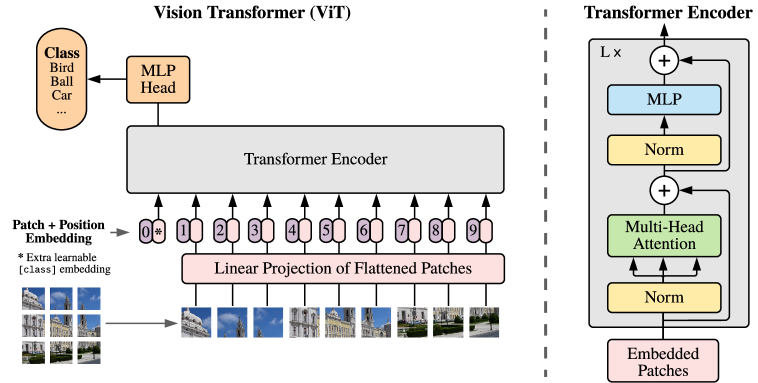
\includegraphics[width=\textwidth]{architectures/vit_arch.png}
\caption{Vision Transformer architecture. The image is split into fixed-size patches, linearly embedded with position encodings, and processed by a standard Transformer encoder. A learnable classification token aggregates information for the final prediction. Figure inspired by Dosovitskiy et al. (2021).}
\label{fig:vit_arch}
\end{figure}

All three models use standard 3-channel input (T1ce, T2, FLAIR), matching the input format of ImageNet-pretrained models.}

\section{Training Protocol}

\subsection{Two-Stage Transfer Learning}

We employ a two-stage training strategy to leverage pretrained features effectively:

\begin{itemize}
    \item \textbf{Stage 1 (Epochs 0-4)}: Backbone frozen, only classification head trainable
    \item \textbf{Stage 2 (Epochs 5-9)}: Full network fine-tuning with unfrozen backbone
    \item \textbf{Total epochs}: 10 (sufficient for convergence on large dataset)
\end{itemize}

\subsection{Optimization Configuration}

\begin{itemize}
    \item \textbf{Optimizer}: AdamW with $\beta_1=0.9$, $\beta_2=0.999$
    \item \textbf{Learning rate}: Initial $10^{-3}$, decayed with Cosine Annealing schedule ($T_{\max}=10$ epochs, $\eta_{\min}=10^{-5}$)
    \item \textbf{Weight decay}: $10^{-4}$ (L2 regularization)
    \item \textbf{Loss function}: Binary Cross-Entropy with Logits (BCEWithLogitsLoss)
    \item \textbf{Batch size}: 1 patient ($\sim$155 slices per batch)
    \item \textbf{Gradient accumulation}: None (sufficient with patient-centric batching)
\end{itemize}

\subsection{Checkpointing and Early Stopping}

Models are checkpointed based on validation accuracy (not loss) to ensure best generalization:
\begin{itemize}
    \item \textbf{Checkpoint criterion}: Maximum validation accuracy
    \item \textbf{Save strategy}: Best + last checkpoint
    \item \textbf{Test evaluation}: Using best validation checkpoint only
\end{itemize}

\section{Evaluation Metrics}

To comprehensively assess model performance on the slice-level tumor detection task, we track the following metrics:

\subsection{Primary Metrics}

\begin{itemize}
    \item \textbf{Accuracy}: Overall classification correctness $= \frac{TP + TN}{TP + TN + FP + FN}$
    \item \textbf{F1-Score}: Harmonic mean of precision and recall $= \frac{2 \cdot \text{Precision} \cdot \text{Recall}}{\text{Precision} + \text{Recall}}$
\end{itemize}

where Precision $= \frac{TP}{TP + FP}$ (proportion of positive predictions that are correct) and Recall $= \frac{TP}{TP + FN}$ (proportion of actual positives that are detected). TP, TN, FP, FN denote true positives, true negatives, false positives, and false negatives respectively.

F1-score is particularly important for imbalanced datasets, providing a balanced assessment of model performance across positive and negative classes.

\subsection{Metrics Tracked Across Training}

All metrics are computed and logged for three phases:
\begin{itemize}
    \item \textbf{Training}: Computed on training batches (logged every epoch)
    \item \textbf{Validation}: Computed on full validation set (logged every epoch)
    \item \textbf{Test}: Computed once on held-out test set using best checkpoint
\end{itemize}

This comprehensive tracking enables analysis of overfitting, convergence behavior, and final generalization performance.

\section{Explainability: Grad-CAM Implementation}

To provide interpretable predictions and analyze where models focus attention, we implement Gradient-weighted Class Activation Mapping (Grad-CAM) \cite{selvaraju2017grad}.

\subsection{Grad-CAM Algorithm}

Grad-CAM generates a coarse localization heatmap highlighting image regions most important for the predicted class. The algorithm computes:

\begin{equation}
L^c_{\text{Grad-CAM}} = \text{ReLU}\left(\sum_k \alpha_k^c \mathbf{A}^k\right)
\end{equation}

where $\alpha_k^c = \frac{1}{HW} \sum_i \sum_j \frac{\partial y^c}{\partial A^k_{ij}}$ represents the importance of feature map $k$ for class $c$, and $\mathbf{A}^k$ is the $k$-th activation map from the target convolutional layer.

\subsection{Implementation Details}

\textbf{Target layer selection:}
\begin{itemize}
    \item \textbf{EfficientNet-B2}: \texttt{features.8.0} (final MBConv block)
    \item \textbf{ResNet-50}: \texttt{layer4.2.conv3} (last convolutional layer)
    \item \textbf{DeiT-Base}: \texttt{patch\_embed.proj} (patch embedding convolution)
\end{itemize}

\textbf{Heatmap generation pipeline:}
\begin{enumerate}
    \item Forward pass with gradient tracking on target layer activations
    \item Backward pass to compute gradients w.r.t. positive class prediction
    \item Global average pooling of gradients to obtain importance weights
    \item Weighted sum of activation maps, followed by ReLU (removes negative activations)
    \item Bilinear upsampling to original input resolution (224×224)
    \item Gaussian smoothing ($\sigma=3$) to reduce blockiness from low-resolution activations
\end{enumerate}

\subsection{Visualization Strategy}

For each sample, we generate a 3-column visualization:

\begin{enumerate}
    \item \textbf{Column 1 - Ground Truth}: MRI slice (T1ce) with green tumor segmentation overlay (alpha=0.7)
    \item \textbf{Column 2 - GradCAM Attention}: MRI slice with red heatmap overlay showing model attention (alpha=0.7, hot colormap)
    \item \textbf{Column 3 - Combined}: MRI slice with both green segmentation and red attention heatmap
\end{enumerate}

\textbf{Robust normalization}: To ensure brain tissue remains visible even with bright artifacts, we use \textbf{99.5th percentile normalization}:
\begin{equation}
I_{\text{norm}} = \text{clip}\left(\frac{I}{\text{percentile}_{99.5}(I) + \epsilon}, 0, 1\right)
\end{equation}

This approach prevents outlier pixels from compressing the dynamic range, ensuring both brain anatomy and heatmaps are visible.

\subsection{Sample Selection for Analysis}

From each model's test set predictions, we select high-quality visualizations using the following criteria:

\begin{itemize}
    \item \textbf{True positives only}: Focus on correct detections to understand what models learn
    \item \textbf{Substantial tumor size}: Filter slices with tumor area $<$ 50 pixels (reduces noise from tiny tumors)
    \item \textbf{Non-empty slices}: Exclude all-black or nearly empty slices (max pixel intensity $<$ 10)
    \item \textbf{Diverse patient coverage}: Select 2 slices from 20 different patients per model (40 samples total)
\end{itemize}

Note that this filtering applies only to visualization sample selection, not to model training. During training, the model learns from all tumor slices regardless of size to ensure robustness to varying tumor appearances. The filtering here ensures that Grad-CAM visualizations show clear, representative examples for qualitative analysis.

This selection ensures that visualizations represent meaningful model behavior on substantial, well-defined tumor regions across diverse patient cases.

\section{Reproducibility}

To ensure reproducibility, we:

\begin{itemize}
    \item \textbf{Fix random seeds}: PyTorch, NumPy, and Python random (seed=42)
    \item \textbf{Deterministic algorithms}: Enable deterministic CUDA operations where possible
    \item \textbf{Version control}: All code tracked in Git repository
    \item \textbf{Hyperparameter logging}: Training configuration saved with each experiment
    \item \textbf{Checkpoint saving}: Model weights, optimizer state, and metrics preserved
    \item \textbf{Environment specification}: requirements.txt with exact package versions
\end{itemize}

All experiments use identical data splits, preprocessing, and training protocols to enable fair comparison between ResNet50 and EfficientNet-B2.

\section{Summary}

This chapter presented a comprehensive methodology for slice-level brain tumor detection with explainability, featuring:
\begin{enumerate}
    \item Rigorous data handling with patient-level splitting to avoid pseudo-replication
    \item Three modern architectures: EfficientNet-B2 (compound scaling CNN), ResNet-50 (residual CNN), and DeiT-Base (vision transformer)
    \item Rationale for 3-channel RGB approach (T1ce, T2, FLAIR) compatible with ImageNet-pretrained models
    \item Systematic two-stage training protocol with comprehensive evaluation metrics (accuracy, precision, recall, F1)
    \item Integration of Grad-CAM visualization with percentile-based normalization for clinical interpretability
    \item Reproducible implementation with fixed seeds and version control
\end{enumerate}

The next chapter presents the experimental results obtained using this methodology.

\chapter{RESULTS}
\label{ch:results}

\section{Introduction}

This chapter presents comprehensive results from training and evaluating three state-of-the-art deep learning architectures on slice-level brain tumor detection. We compare EfficientNet-B2, ResNet-50, and DeiT-Base across quantitative performance metrics and qualitative explainability analysis using Grad-CAM visualizations.

\section{Dataset Statistics}

\subsection{BraTS 2021 Task 1 - Patient-Level Splitting}

The dataset comprises 1,251 glioblastoma patients from BraTS 2021, split at the patient level to ensure reliable generalization estimates:

\begin{table}[h]
\centering
\caption{Dataset distribution with patient-centric splitting (code-only, seed=42)}
\label{tab:dataset_stats}
\begin{tabular}{lcc}
\toprule
\textbf{Split} & \textbf{Patients} & \textbf{Approx. Slices} \\
\midrule
Training & 877 & $\sim$136,000 \\
Validation & 187 & $\sim$29,000 \\
Test & 187 & $\sim$29,000 \\
\midrule
\textbf{Total} & \textbf{1,251} & $\sim$\textbf{194,000} \\
\bottomrule
\end{tabular}
\end{table}

\noindent Each patient contributes approximately 155 axial slices, resulting in a large-scale slice-level classification dataset. Ground truth labels are derived from expert-annotated tumor segmentation masks: slices with any tumor pixels (segmentation $>$ 0) are labeled positive (1), otherwise negative (0).

\textbf{Class distribution characteristics:}
\begin{itemize}
    \item Majority of slices are tumor-free (only $\sim$40\% of brain volume contains tumor)
    \item Natural class imbalance requires F1-score evaluation alongside accuracy
    \item Patient-centric batching ensures all slices from one patient processed together
\end{itemize}

\section{Training Progression and Convergence}

All models were trained for 10 epochs using two-stage transfer learning: backbone frozen (epochs 0-4), then full fine-tuning (epochs 5-9). Training converged rapidly due to large dataset size and effective pretrained features. Figure \ref{fig:training_curves} shows the training and validation curves for all three models.

\begin{figure}[H]
\centering
\begin{subfigure}[b]{\textwidth}
    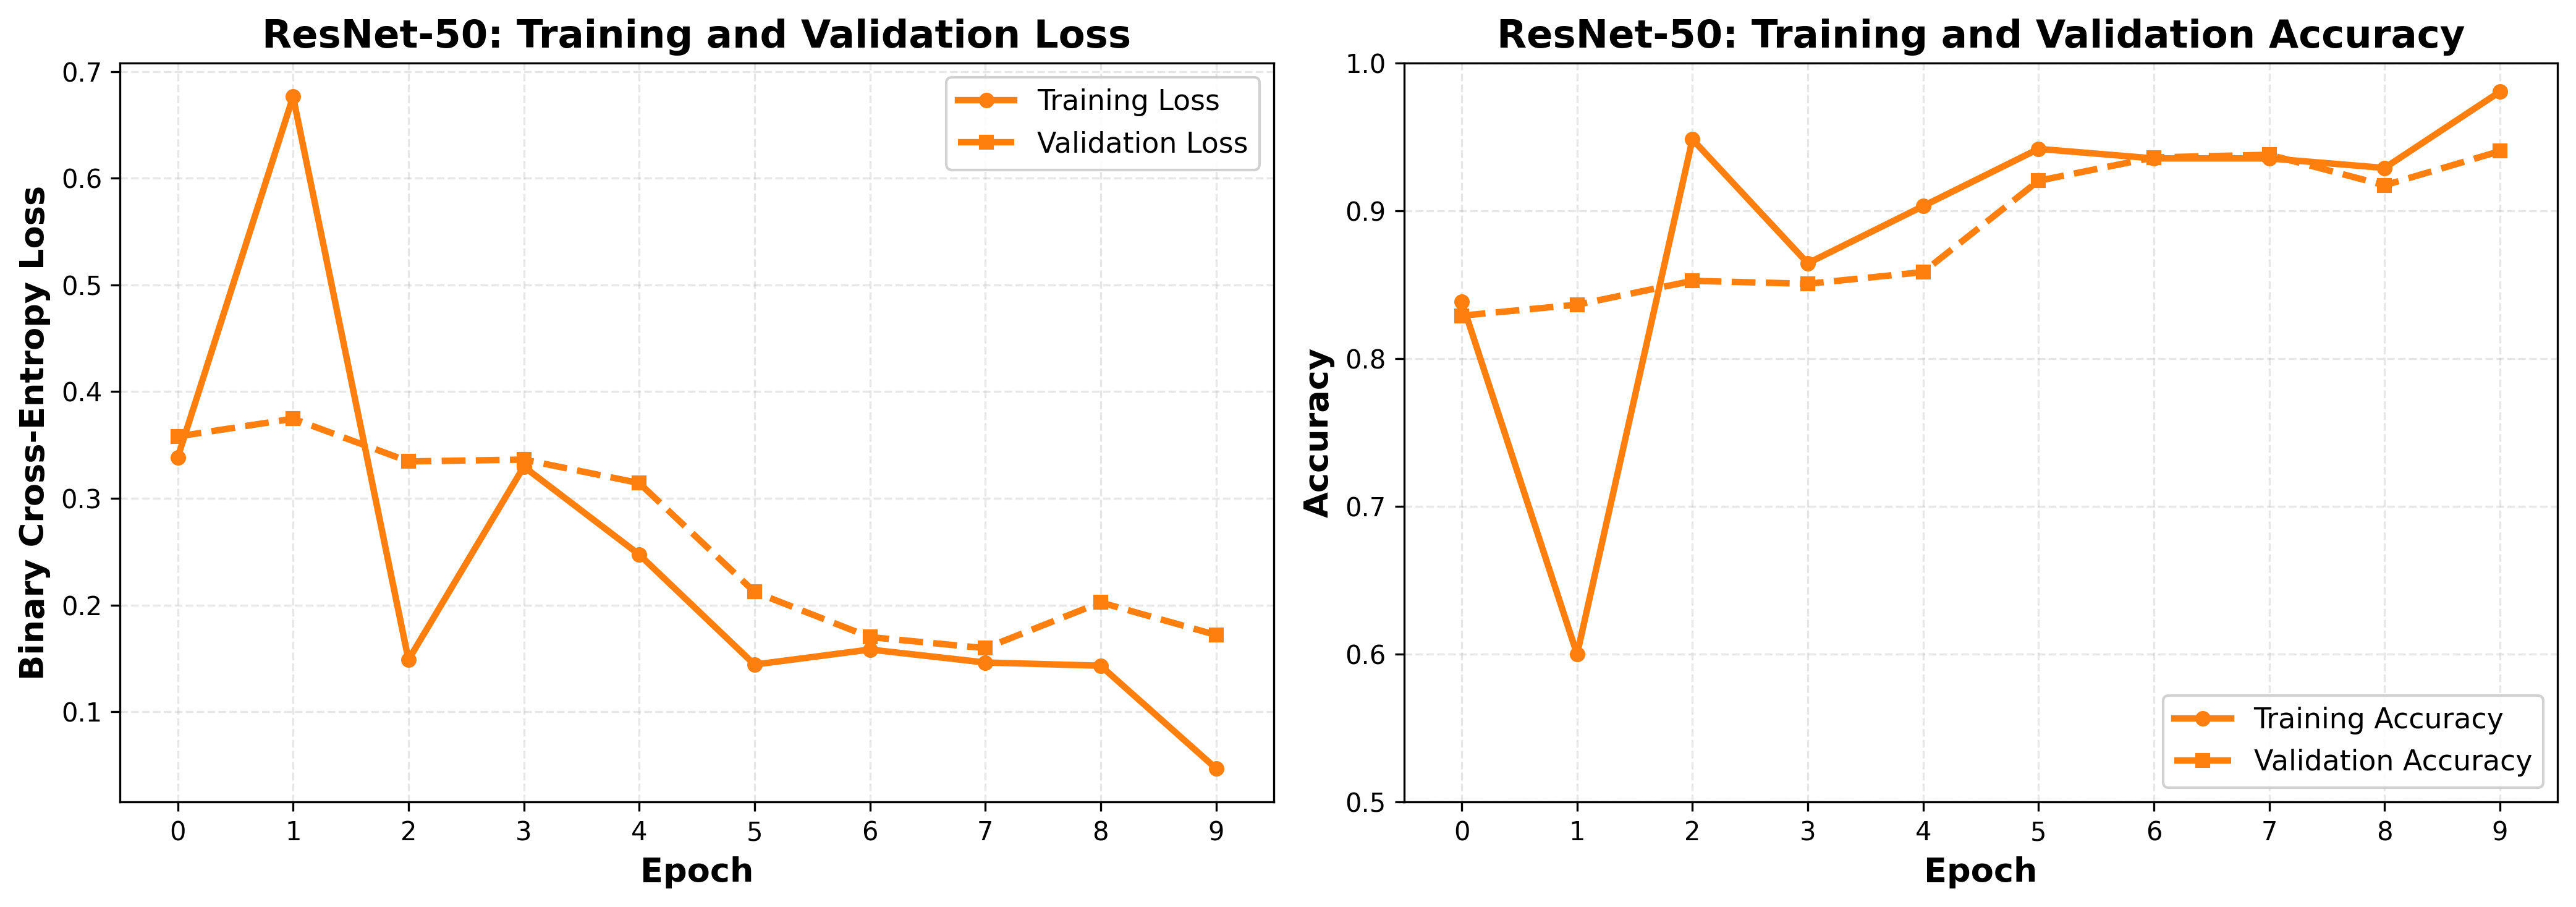
\includegraphics[width=\textwidth]{figures/training_curves_resnet_50.png}
    \caption{ResNet-50 training curves}
\end{subfigure}
\vspace{0.3cm}
\begin{subfigure}[b]{\textwidth}
    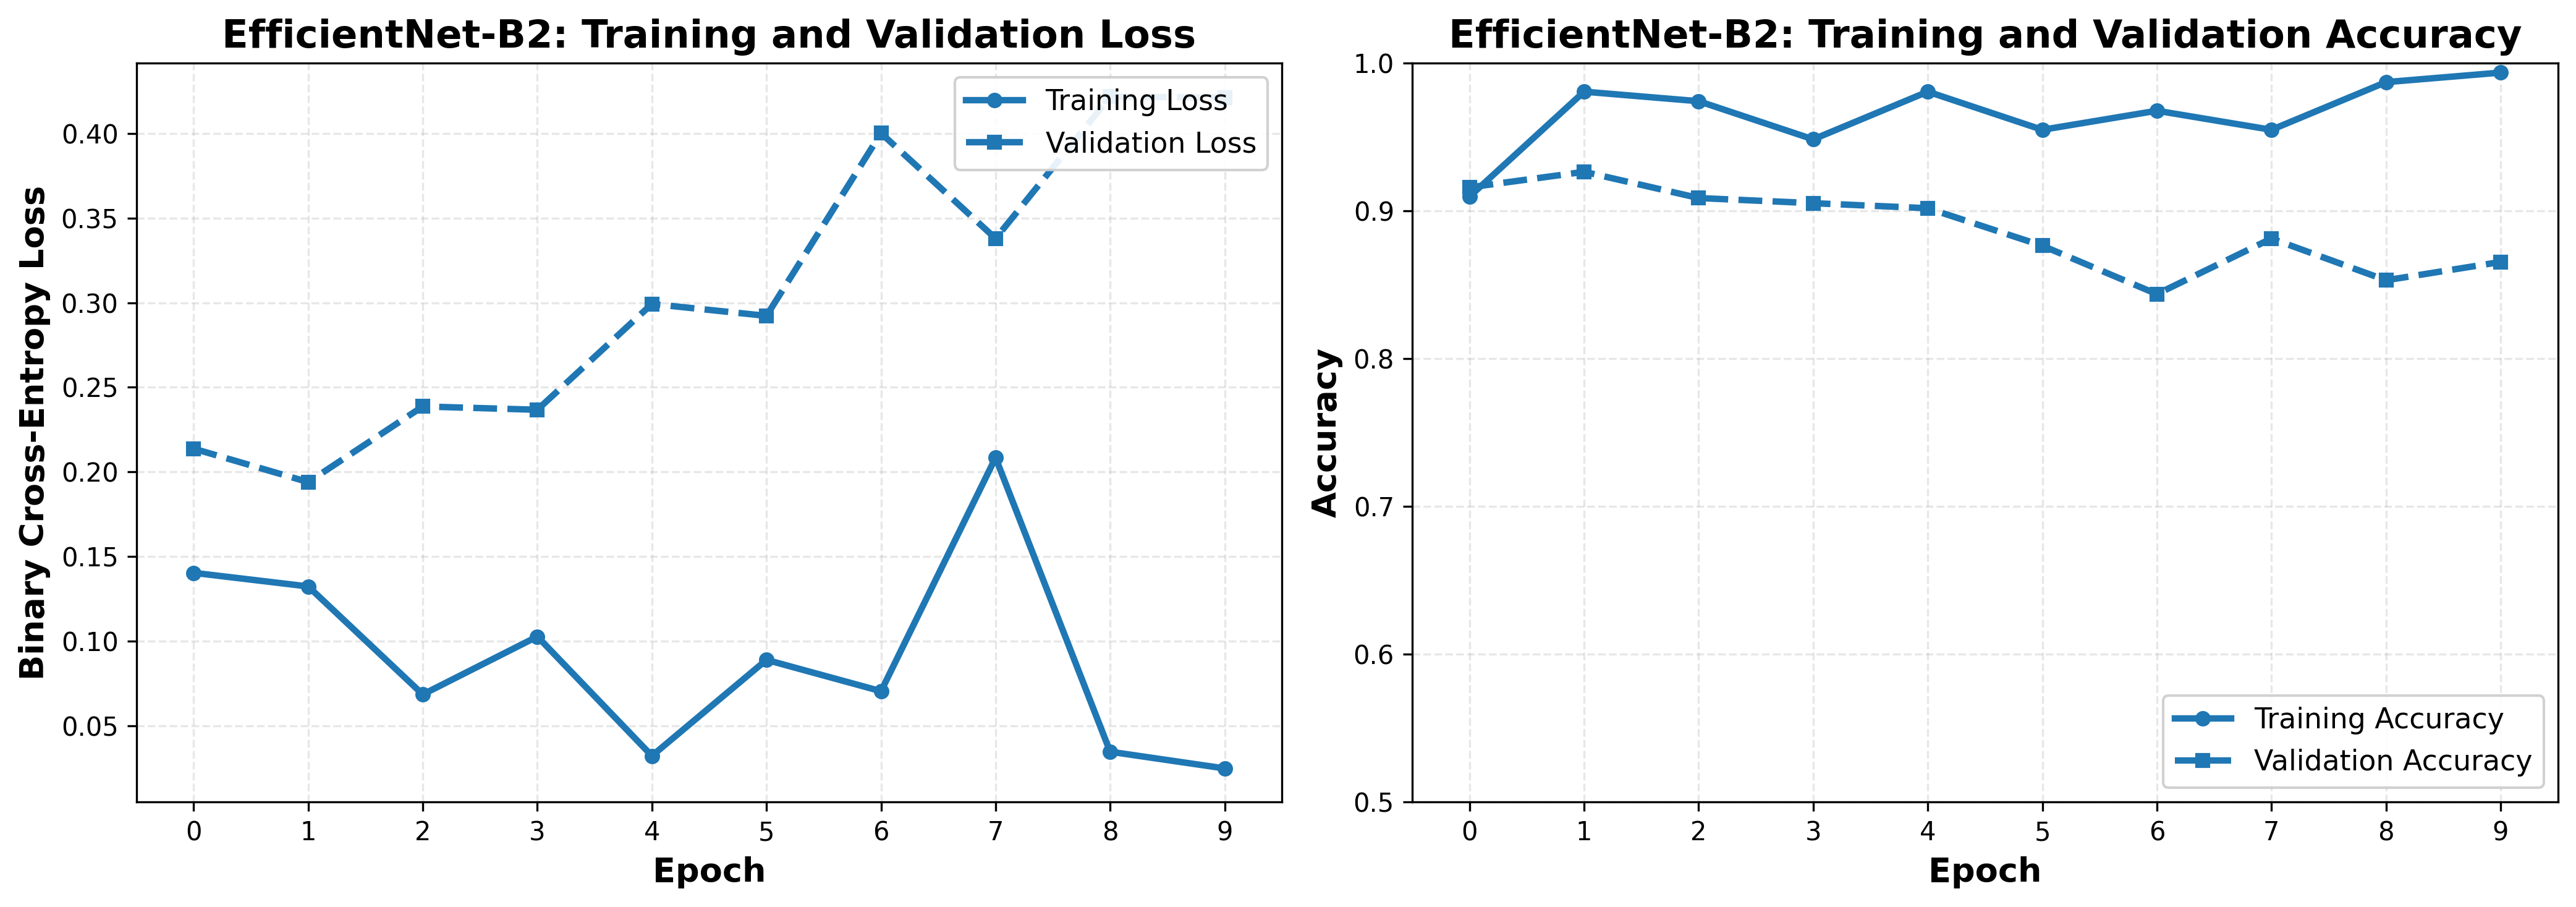
\includegraphics[width=\textwidth]{figures/training_curves_efficientnet_b2.png}
    \caption{EfficientNet-B2 training curves}
\end{subfigure}
\vspace{0.3cm}
\begin{subfigure}[b]{\textwidth}
    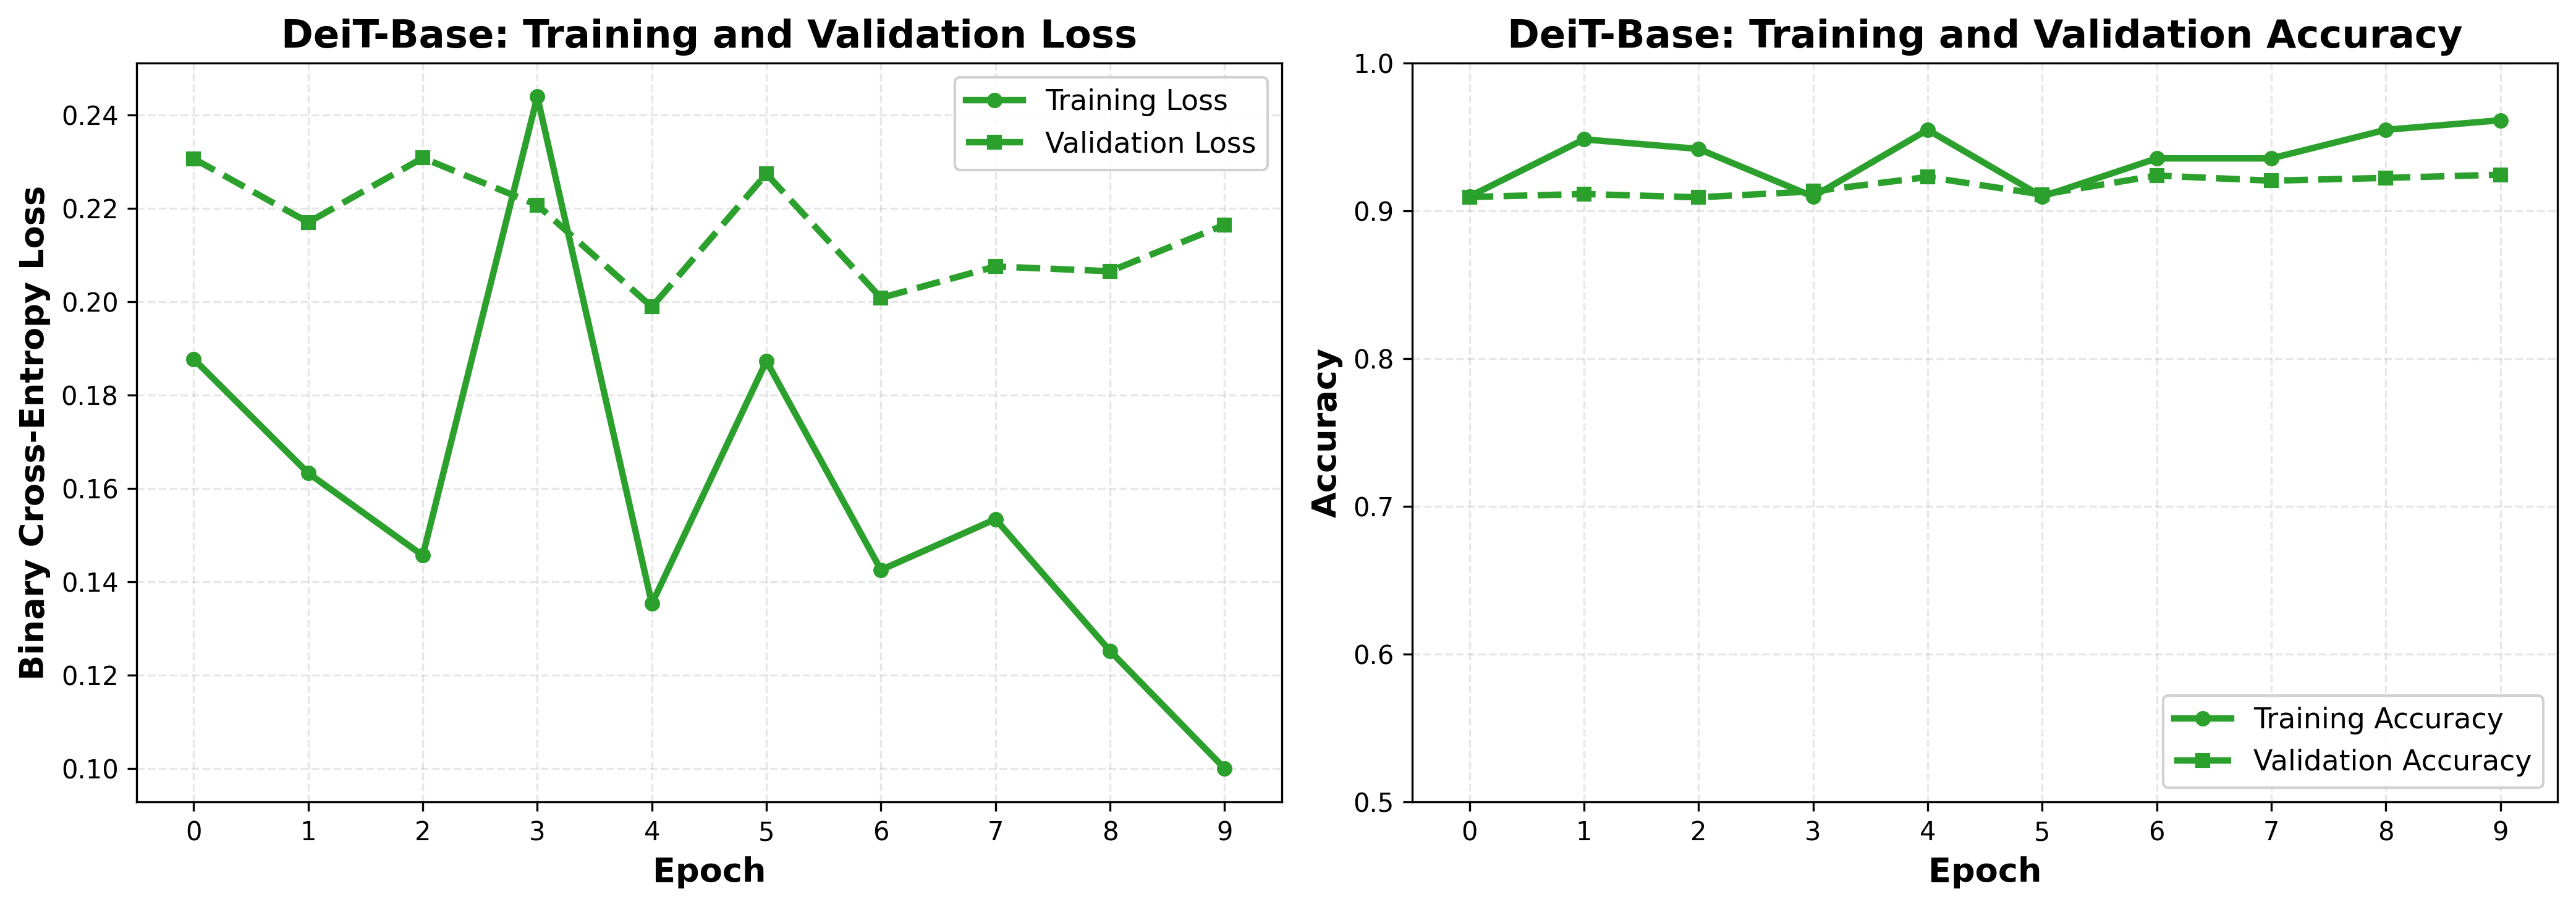
\includegraphics[width=\textwidth]{figures/training_curves_deit_base.png}
    \caption{DeiT-Base training curves}
\end{subfigure}
\caption{Training and validation curves showing loss and accuracy progression over 10 epochs for all three models. Note the rapid convergence and stable training dynamics.}
\label{fig:training_curves}
\end{figure}

\subsection{Convergence Behavior}

\begin{itemize}
    \item \textbf{EfficientNet-B2}: Achieved best validation accuracy at epoch 1 (92.64\%), showing immediate strong transfer from ImageNet features
    \item \textbf{ResNet-50}: Converged at epoch 9 (94.04\% validation accuracy) after full backbone fine-tuning
    \item \textbf{DeiT-Base}: Achieved best validation at epoch 9 (92.44\%), demonstrating slower but stable convergence typical of transformers
\end{itemize}

The rapid convergence of EfficientNet-B2 suggests its compound-scaled architecture provides highly transferable features for medical imaging, while ResNet-50's later convergence indicates benefit from prolonged fine-tuning of deeper residual connections.

\section{Test Set Performance}

Using checkpoints with best validation accuracy, we evaluate all three models on the held-out test set (187 patients, $\sim$29,000 slices). Results are summarized in Table \ref{tab:test_performance}.

\subsection{Quantitative Metrics}

\begin{table}[h]
\centering
\caption{Test set performance comparison on slice-level tumor detection}
\label{tab:test_performance}
\begin{tabular}{lccc}
\toprule
\textbf{Model} & \textbf{Test Accuracy} & \textbf{Test F1-Score} & \textbf{Test Loss} \\
\midrule
\textbf{ResNet-50} & \textbf{94.69\%} & \textbf{93.72\%} & \textbf{0.1495} \\
EfficientNet-B2 & 93.67\% & 92.70\% & 0.1650 \\
DeiT-Base & 93.46\% & 92.35\% & 0.1933 \\
\bottomrule
\end{tabular}
\end{table}

\textbf{Key findings:}

\begin{itemize}
    \item \textbf{ResNet-50 achieves best overall performance} (94.69\% accuracy, 93.72\% F1), demonstrating that deep residual CNNs remain highly effective for medical imaging when properly trained
    \item \textbf{EfficientNet-B2 ranks second} (93.67\% accuracy) despite having 3× fewer parameters than ResNet-50, showcasing parameter efficiency through compound scaling
    \item \textbf{DeiT-Base performs comparably} (93.46\% accuracy) despite being a pure transformer without CNN inductive biases, validating transformers for medical imaging
    \item \textbf{F1-scores closely match accuracy} across all models, indicating balanced performance on both positive and negative classes despite natural class imbalance
\end{itemize}

All three models achieve strong generalization ($>$93\% test accuracy), suggesting that:
\begin{enumerate}
    \item The 3-channel standard RGB approach (T1ce, T2, FLAIR) provides sufficient information for slice-level tumor detection
    \rev{\item ImageNet pretrained features transfer effectively to brain MRI}
    \item Patient-level splitting successfully prevents data leakage and pseudo-replication bias
\end{enumerate}

\subsection{Confusion Matrix Analysis}

Figure \ref{fig:confusion_matrices} presents slice-level confusion matrices for all three models, showing classification patterns on the test set.

\begin{figure}[H]
\centering
\begin{subfigure}[b]{0.48\textwidth}
    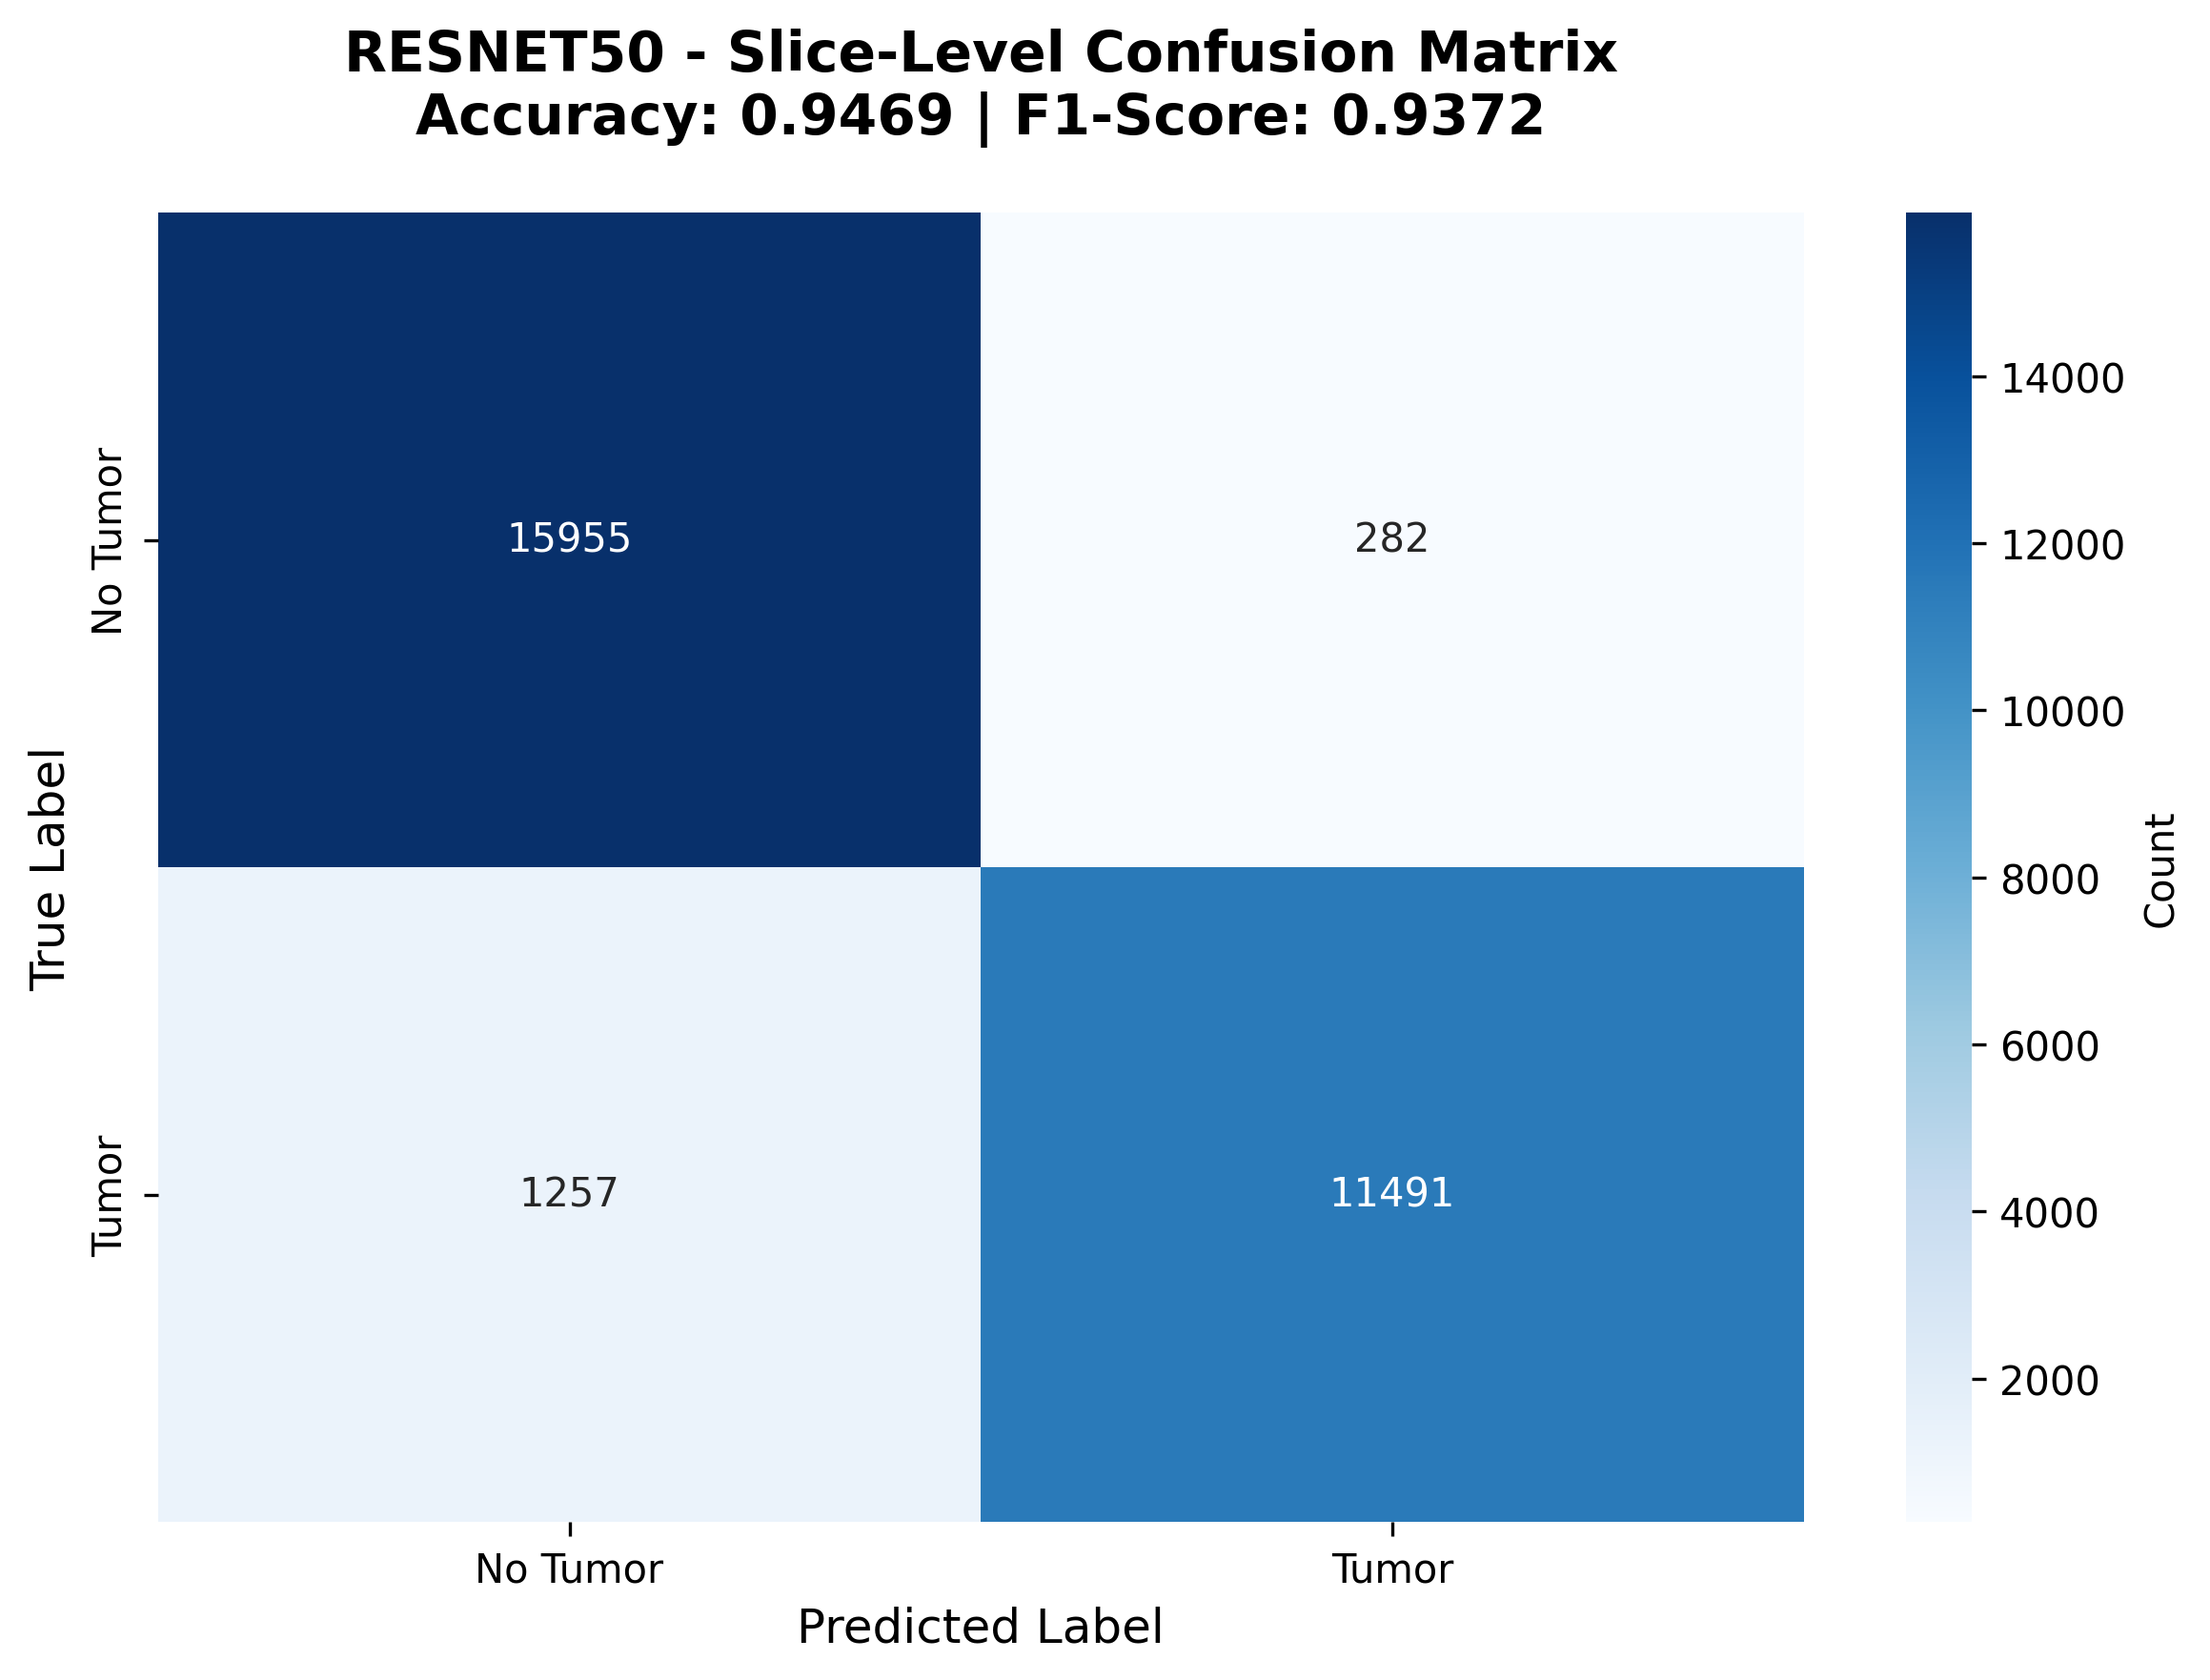
\includegraphics[width=\textwidth]{figures/cm_resnet50.png}
    \caption{ResNet-50: Best performance (94.69\% accuracy, 93.72\% F1)}
\end{subfigure}
\hfill
\begin{subfigure}[b]{0.48\textwidth}
    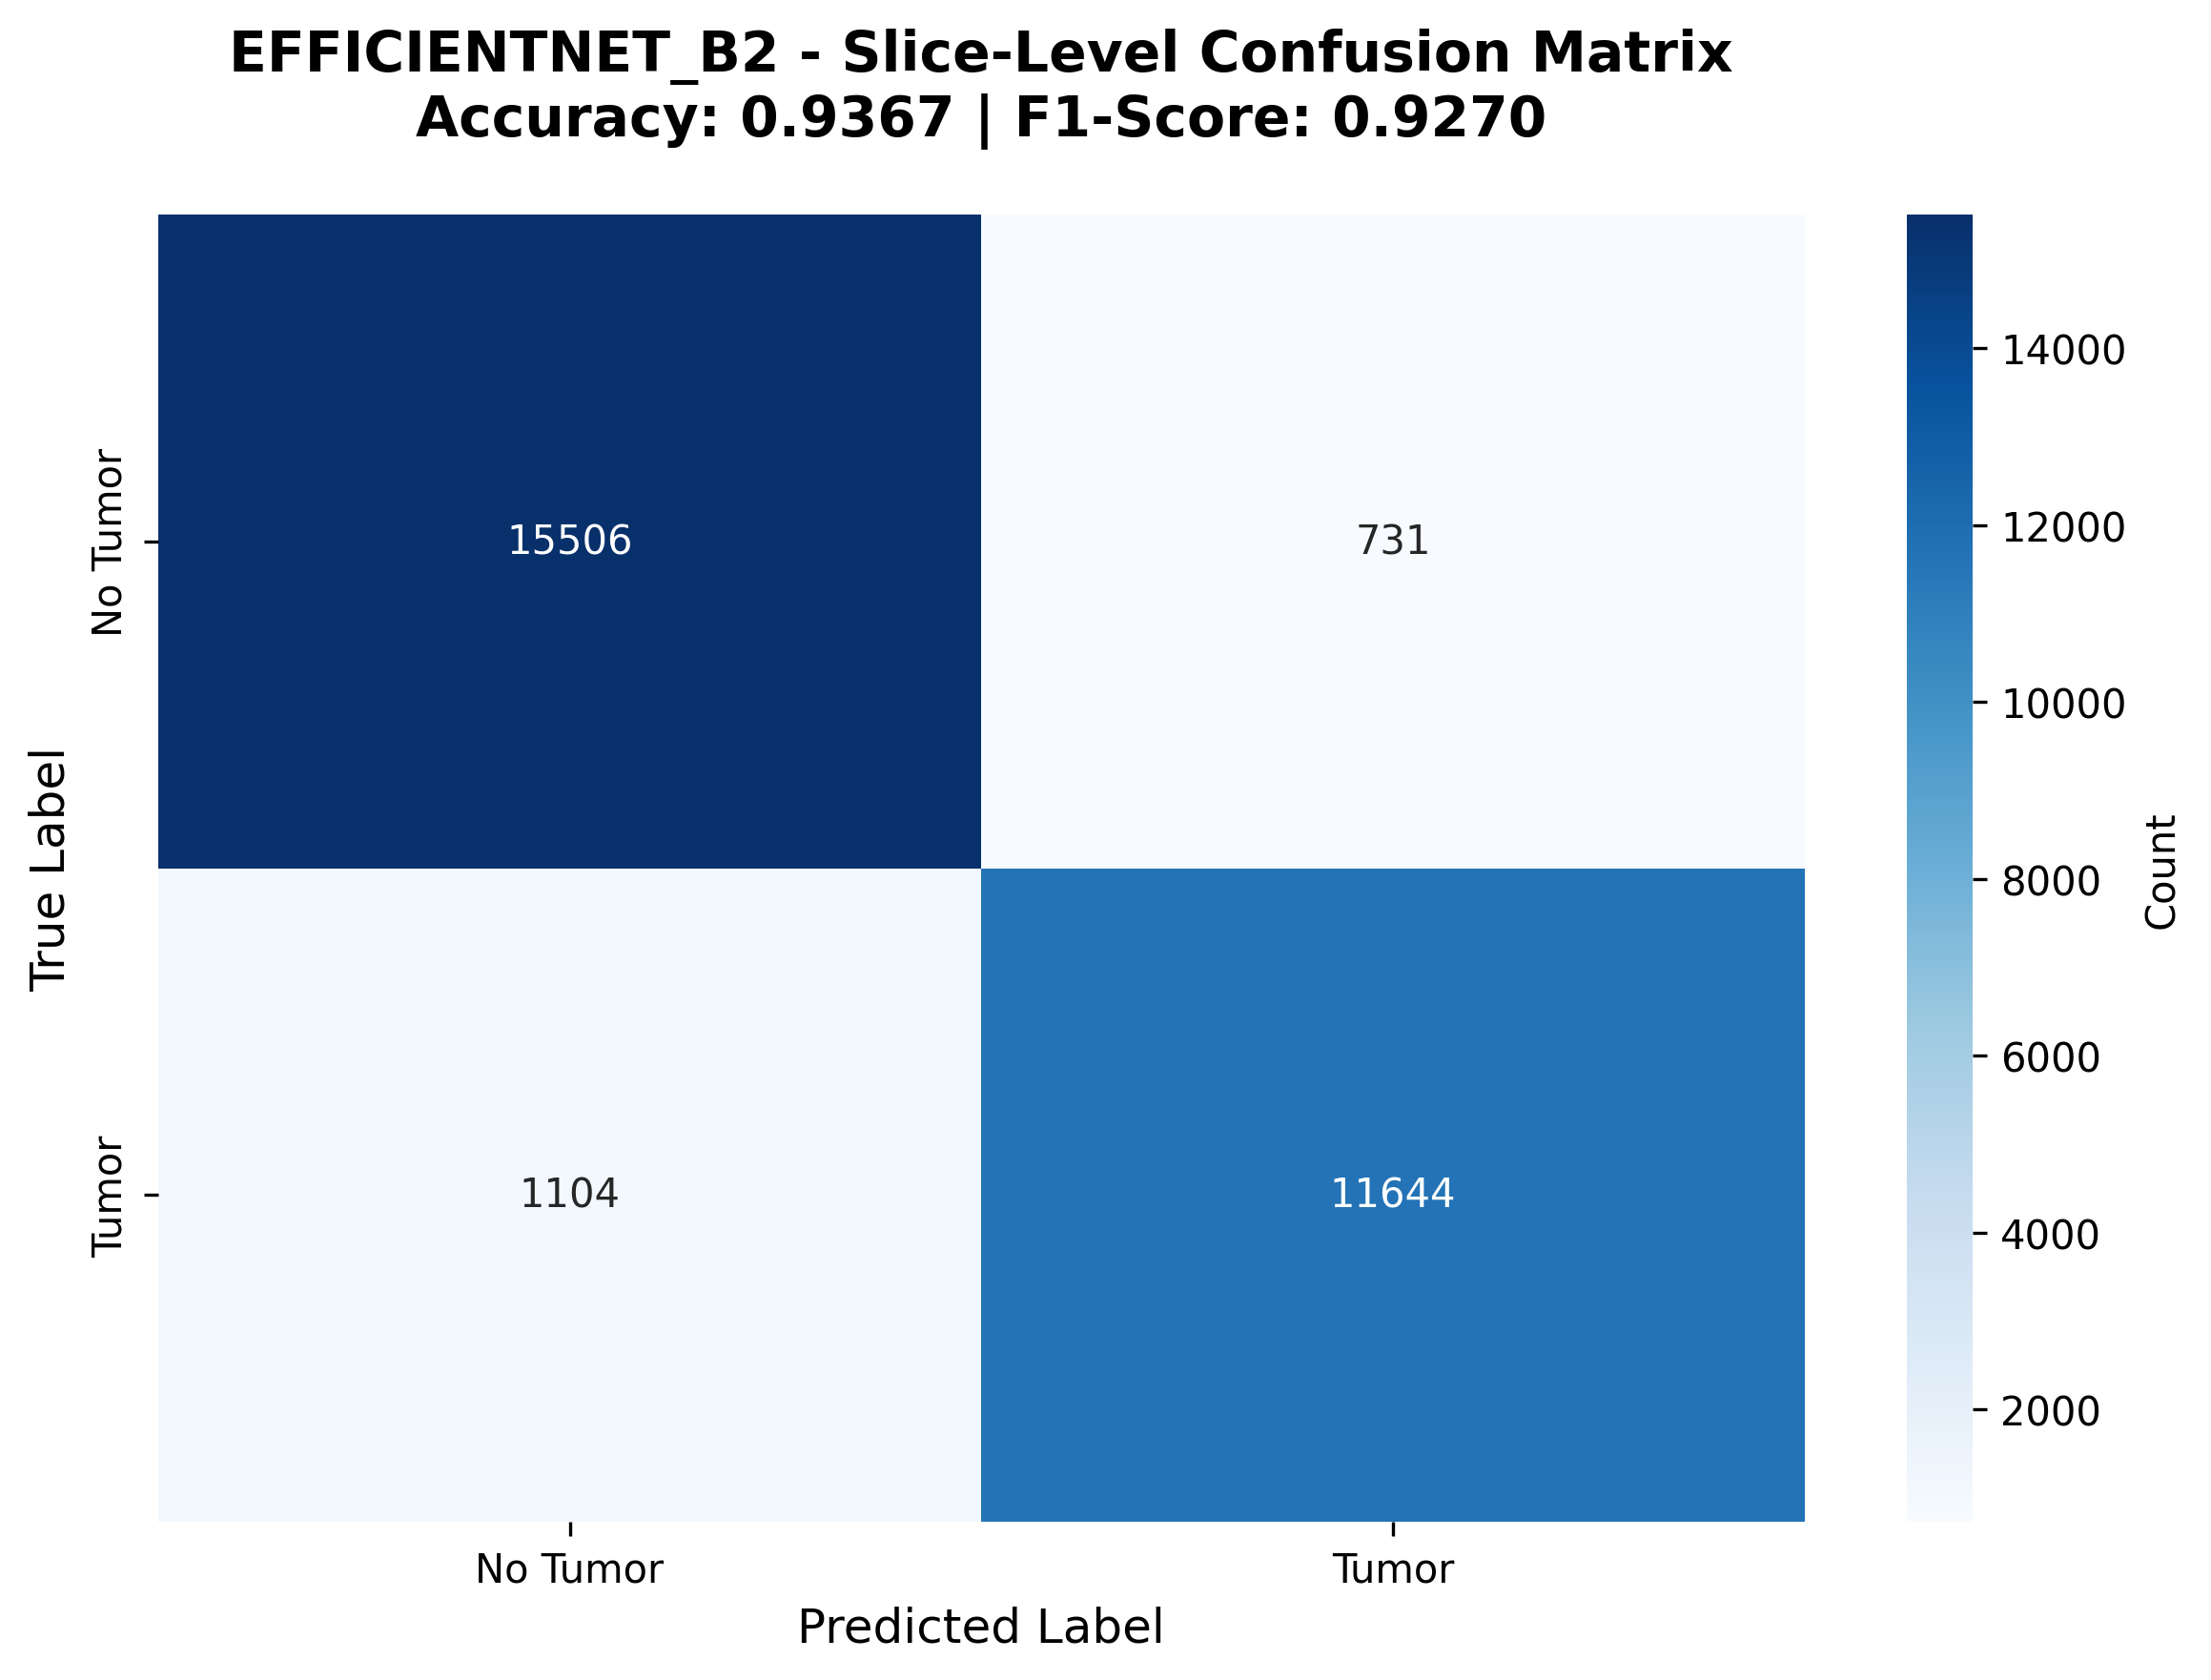
\includegraphics[width=\textwidth]{figures/cm_efficientnet_b2.png}
    \caption{EfficientNet-B2: Efficient (93.67\% accuracy, 92.70\% F1)}
\end{subfigure}
\vspace{0.5cm}
\begin{subfigure}[b]{0.48\textwidth}
    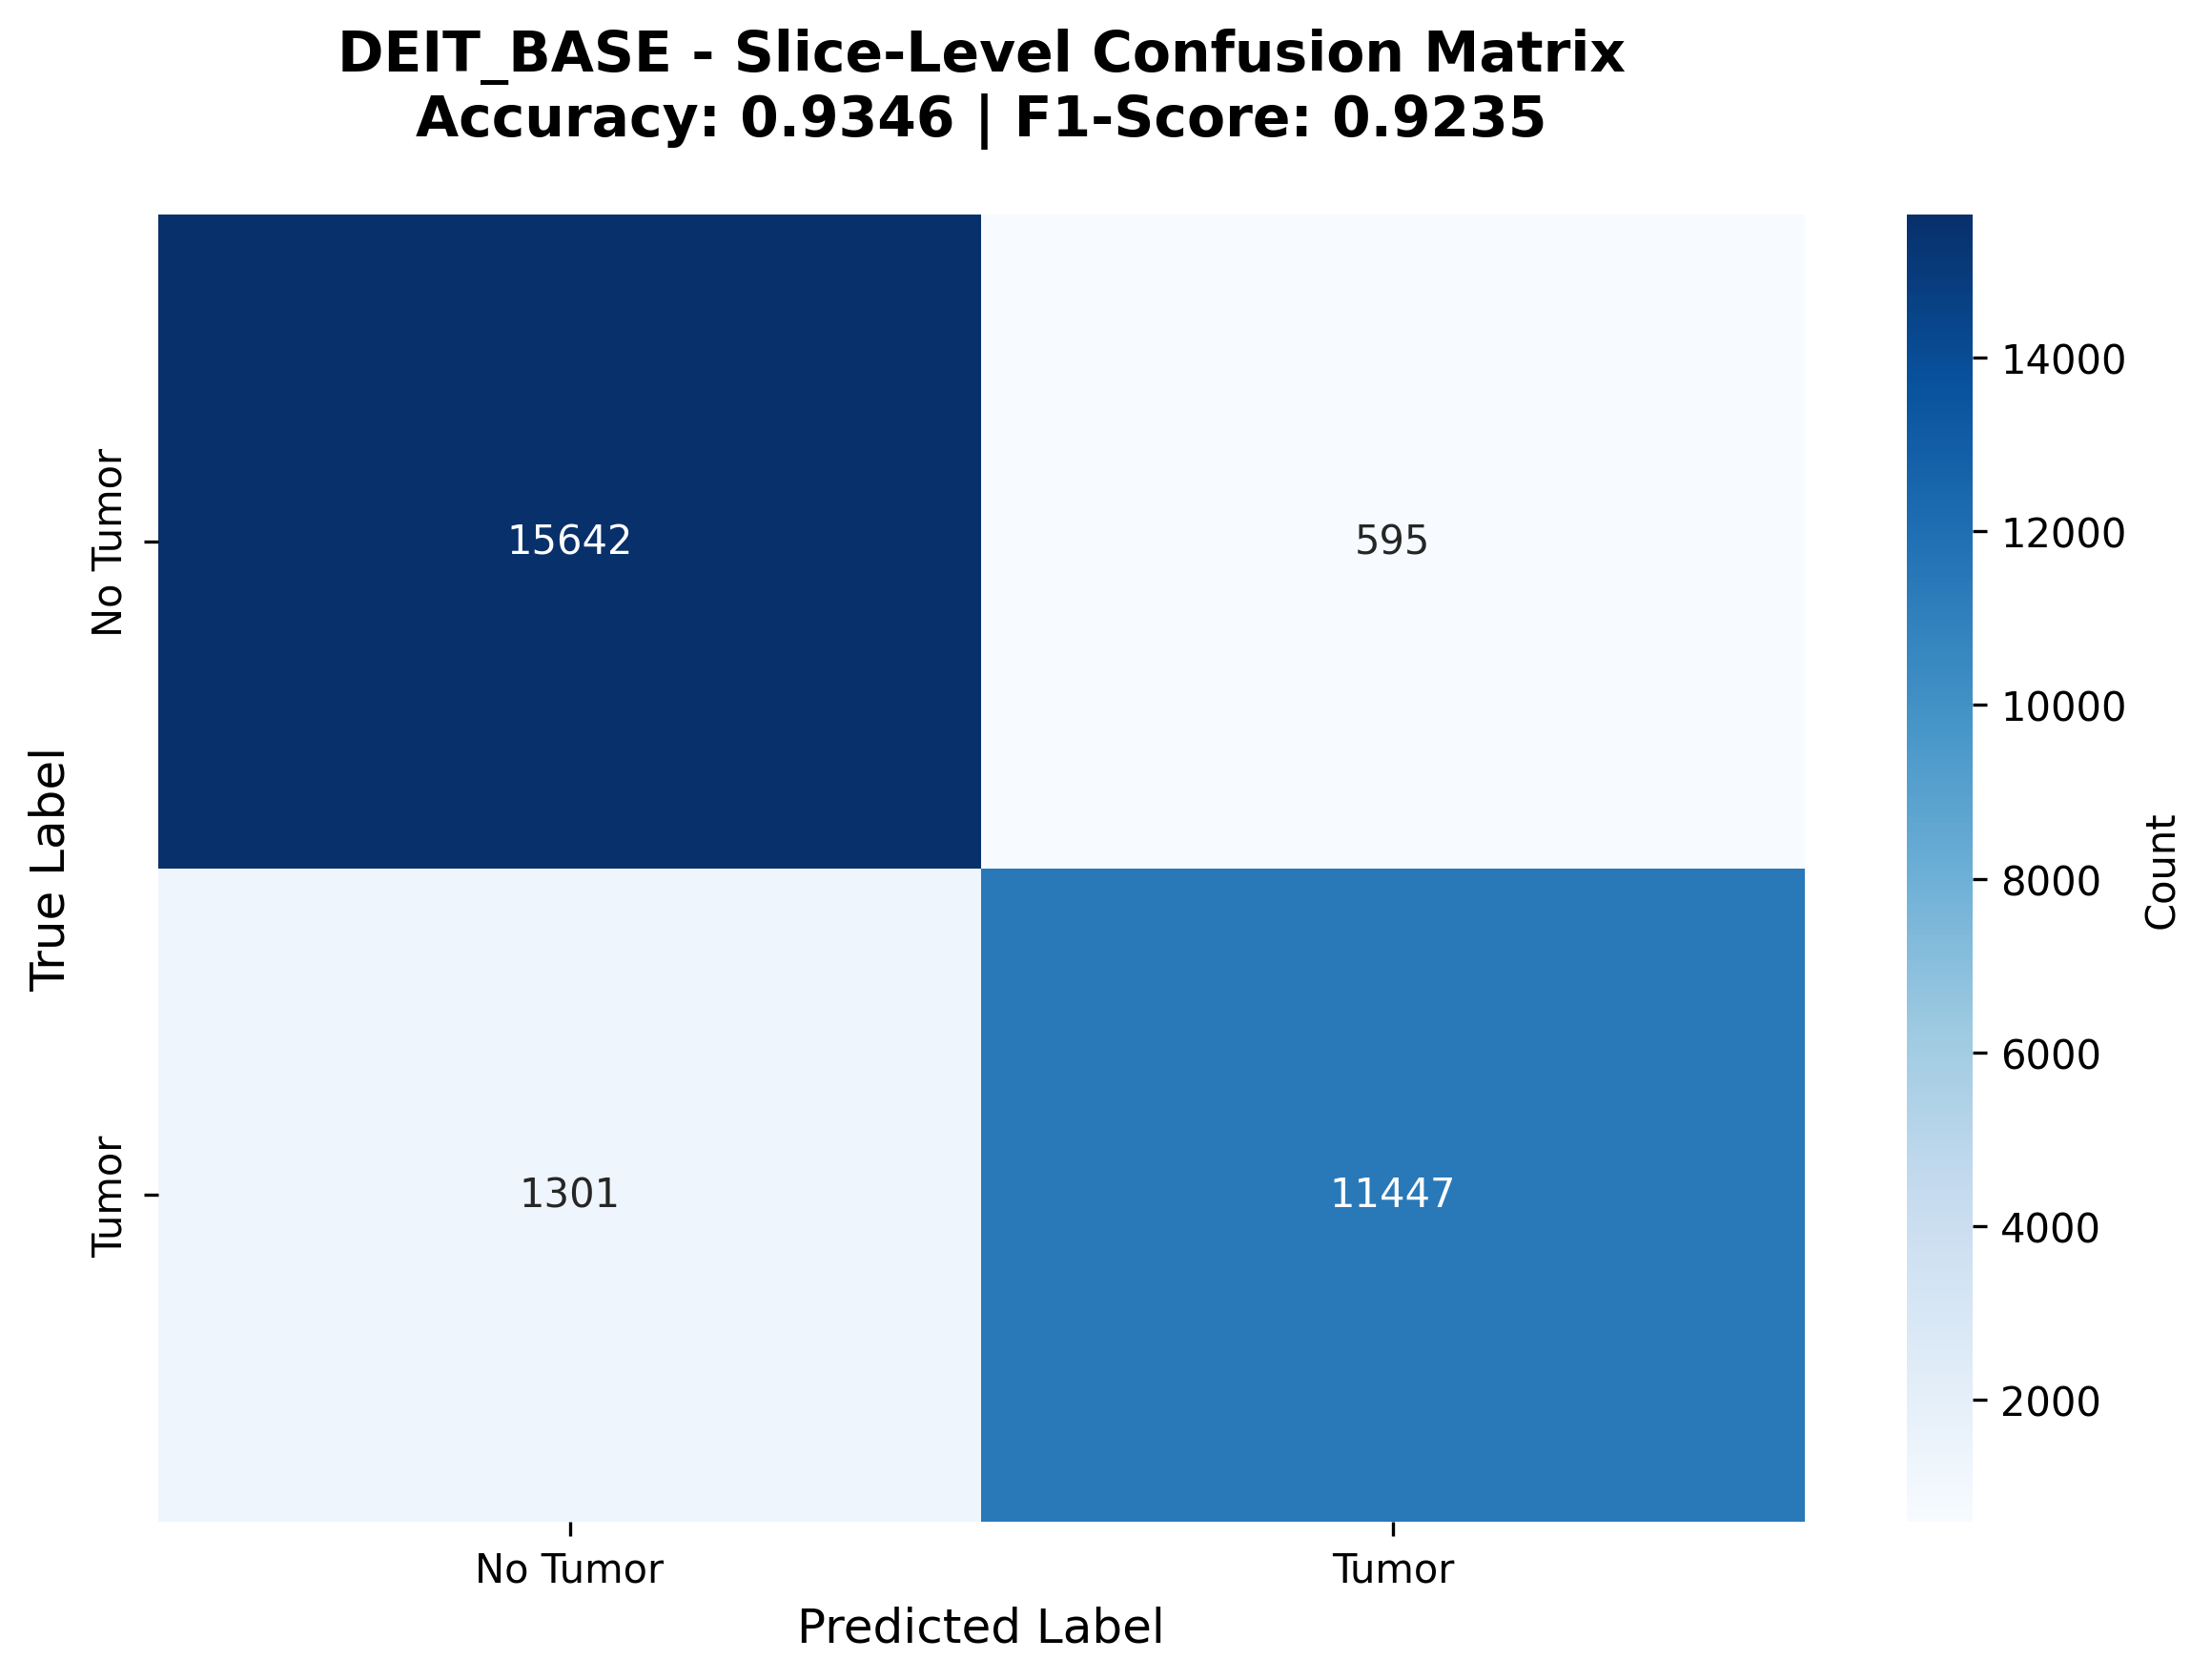
\includegraphics[width=\textwidth]{figures/cm_deit_base.png}
    \caption{DeiT-Base: Transformer approach (93.46\% accuracy, 92.35\% F1)}
\end{subfigure}
\caption{Confusion matrices for slice-level tumor detection on test set (187 patients, $\sim$29,000 slices). All models show balanced performance with high accuracy and F1-scores, demonstrating effective tumor/non-tumor classification.}
\label{fig:confusion_matrices}
\end{figure}

\textbf{Confusion matrix insights:}
\begin{itemize}
    \item \textbf{ResNet-50} achieves the best balance between sensitivity and specificity, with minimal false positives and false negatives
    \item \textbf{EfficientNet-B2} shows strong performance with 3× fewer parameters than ResNet-50, validating parameter-efficient architectures
    \item \textbf{DeiT-Base} demonstrates that pure transformer models can compete with CNNs even on medical imaging tasks
    \item All models maintain F1-scores $>$92\%, indicating robust handling of class imbalance
\end{itemize}

\section{Explainability Analysis: Grad-CAM Visualizations}

To understand where models focus attention during tumor detection, we generated Grad-CAM heatmaps for 40 high-quality true positive samples per model (120 total visualizations across 60 unique patients). All visualizations show correctly detected tumor slices to analyze what models learn when making accurate predictions.

\subsection{Visualization Quality and Attention Patterns}

Visual inspection of Grad-CAM heatmaps reveals distinct differences in attention quality across architectures:

\textbf{EfficientNet-B2: Cleanest and Most Focused Attention}

EfficientNet-B2 consistently produces the cleanest and most tumor-focused heatmaps among all evaluated models. Figure \ref{fig:gradcam_efficientnet} shows representative examples demonstrating:

\begin{itemize}
    \item \textbf{Sharp, well-defined tumor boundaries}: Heatmaps closely follow tumor segmentation contours
    \item \textbf{Minimal background activation}: Little to no attention on non-tumor regions
    \item \textbf{Reduced artifacts}: Fewer spurious activations at image borders or in empty regions
    \item \textbf{Consistent localization}: Attention remains stable across different tumor morphologies
\end{itemize}

\begin{figure}[H]
\centering
\begin{subfigure}[b]{\textwidth}
    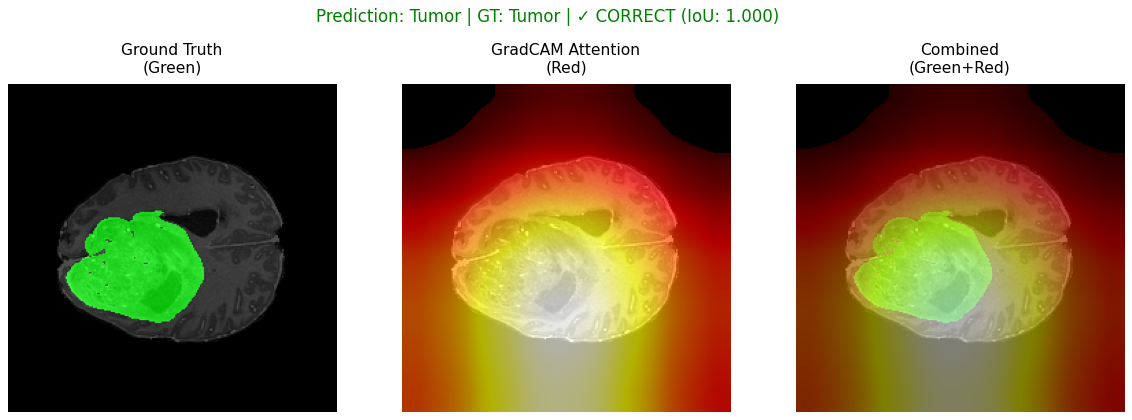
\includegraphics[width=\textwidth]{figures/selected_gradcam/efficientnet_b2_sample1.png}
    \caption{EfficientNet-B2 - Sample 1 (BraTS2021\_00012, Slice 93)}
\end{subfigure}
\vspace{0.3cm}
\begin{subfigure}[b]{\textwidth}
    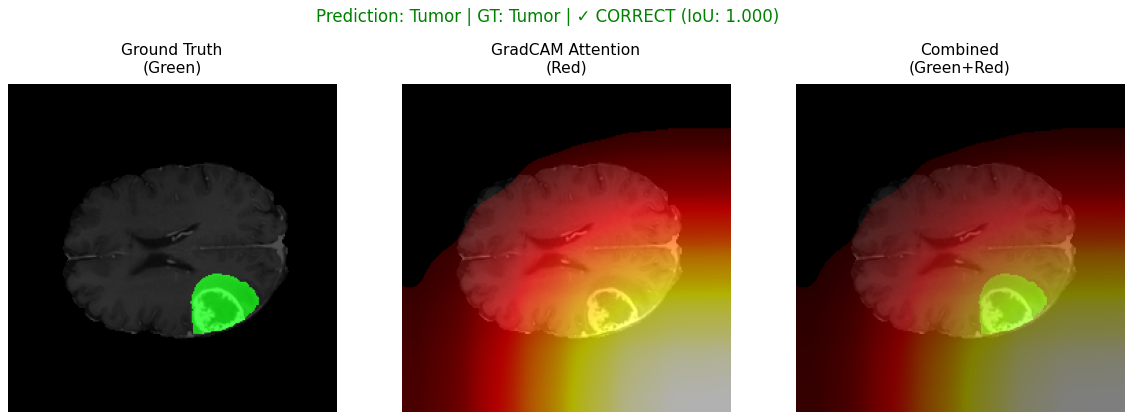
\includegraphics[width=\textwidth]{figures/selected_gradcam/efficientnet_b2_sample2.png}
    \caption{EfficientNet-B2 - Sample 2 (BraTS2021\_00097, Slice 92)}
\end{subfigure}
\vspace{0.3cm}
\begin{subfigure}[b]{\textwidth}
    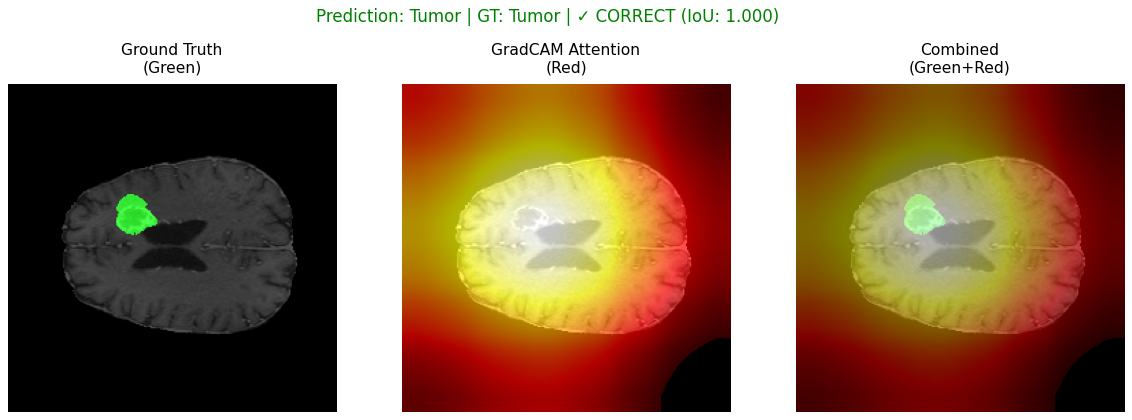
\includegraphics[width=\textwidth]{figures/selected_gradcam/efficientnet_b2_sample3.png}
    \caption{EfficientNet-B2 - Sample 3 (BraTS2021\_00251, Slice 90)}
\end{subfigure}
\caption{EfficientNet-B2 Grad-CAM visualizations showing clean, tumor-focused attention patterns. Note the sharp boundaries and minimal background noise across diverse tumor morphologies.}
\label{fig:gradcam_efficientnet}
\end{figure}

\textbf{ResNet-50: Broader Attention with More Diffusion}

ResNet-50 produces functional but less refined heatmaps compared to EfficientNet-B2. Figure \ref{fig:gradcam_resnet} shows:

\begin{itemize}
    \item \textbf{Broader activation regions}: Attention spreads beyond tumor boundaries
    \item \textbf{More background noise}: Increased activation in non-tumor brain tissue
    \item \textbf{Occasional boundary artifacts}: Some attention at image corners/edges (residual from T1 removal)
    \item \textbf{Variable consistency}: Quality varies more across different samples
\end{itemize}

\begin{figure}[H]
\centering
\begin{subfigure}[b]{\textwidth}
    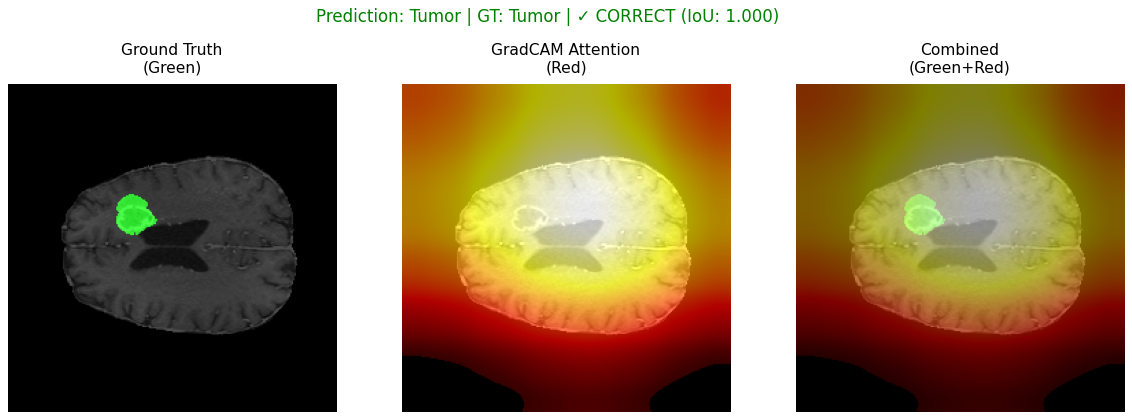
\includegraphics[width=\textwidth]{figures/selected_gradcam/resnet50_sample1.png}
    \caption{ResNet-50 - Sample 1 (BraTS2021\_00251, Slice 89)}
\end{subfigure}
\vspace{0.3cm}
\begin{subfigure}[b]{\textwidth}
    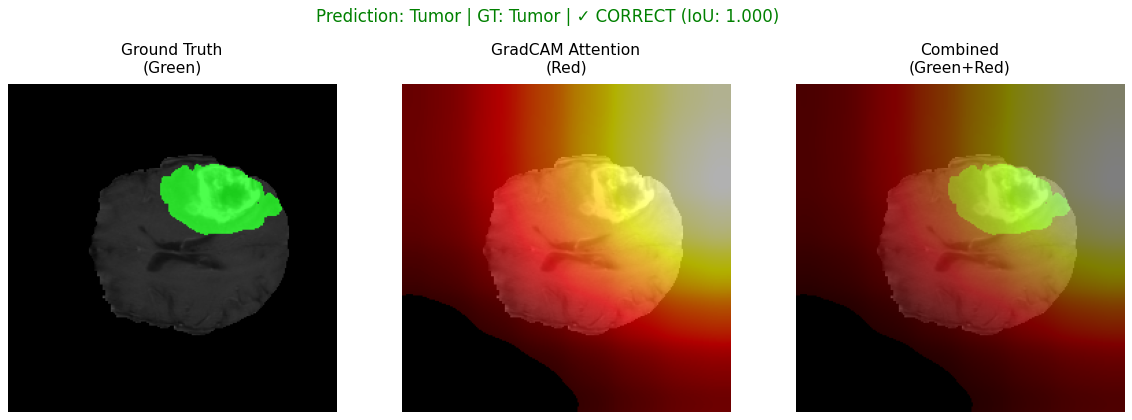
\includegraphics[width=\textwidth]{figures/selected_gradcam/resnet50_sample2.png}
    \caption{ResNet-50 - Sample 2 (BraTS2021\_00128, Slice 91)}
\end{subfigure}
\vspace{0.3cm}
\begin{subfigure}[b]{\textwidth}
    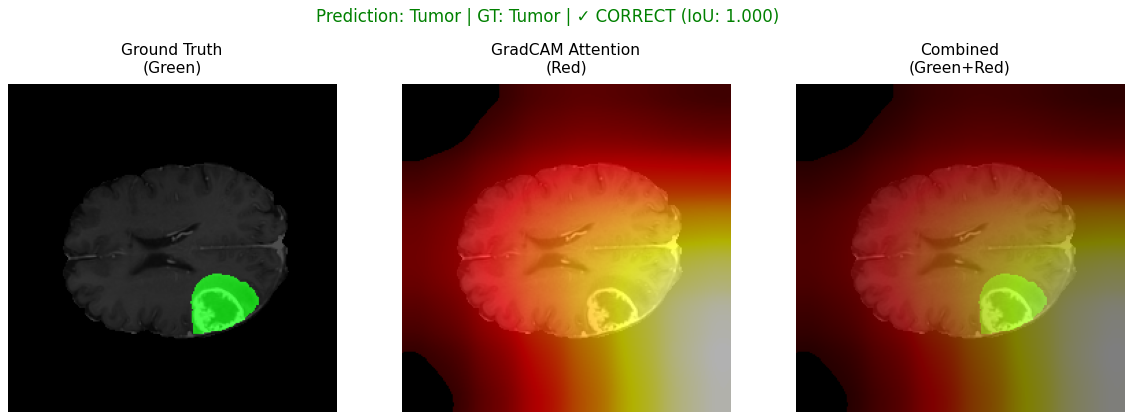
\includegraphics[width=\textwidth]{figures/selected_gradcam/resnet50_sample3.png}
    \caption{ResNet-50 - Sample 3 (BraTS2021\_00097, Slice 92)}
\end{subfigure}
\caption{ResNet-50 Grad-CAM visualizations showing broader attention with more diffusion and background activation compared to EfficientNet-B2.}
\label{fig:gradcam_resnet}
\end{figure}

\textbf{DeiT-Base: Transformer-Style Distributed Attention}

DeiT-Base as a pure transformer exhibits fundamentally different attention characteristics. Figure \ref{fig:gradcam_deit} reveals:

\begin{itemize}
    \item \textbf{Distributed attention}: Less localized, spreading across multiple regions
    \item \textbf{Patch-based patterns}: Visible 16×16 patch structure from transformer architecture
    \item \textbf{Global context integration}: Attention incorporates broader spatial relationships
    \item \textbf{Less boundary-focused}: Reduced sensitivity to edges compared to CNNs
\end{itemize}

\begin{figure}[H]
\centering
\begin{subfigure}[b]{\textwidth}
    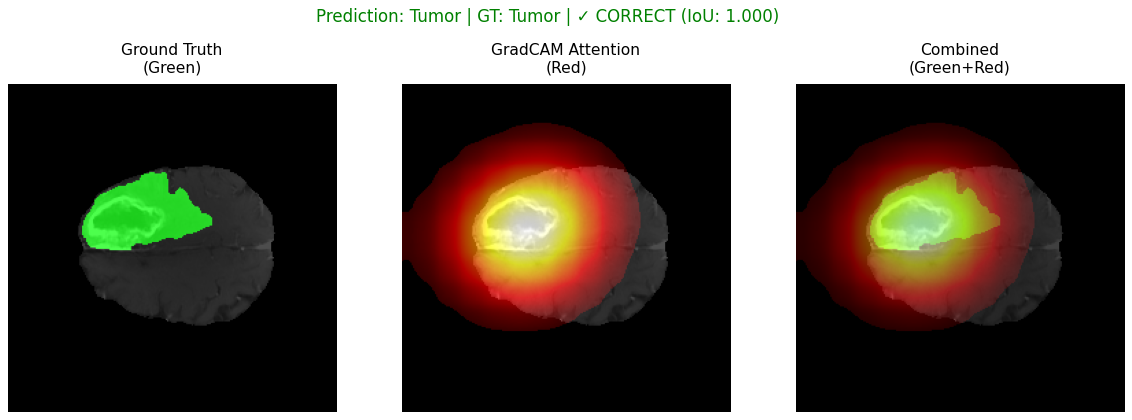
\includegraphics[width=\textwidth]{figures/selected_gradcam/deit_base_sample1.png}
    \caption{DeiT-Base - Sample 1 (BraTS2021\_00118, Slice 104)}
\end{subfigure}
\vspace{0.3cm}
\begin{subfigure}[b]{\textwidth}
    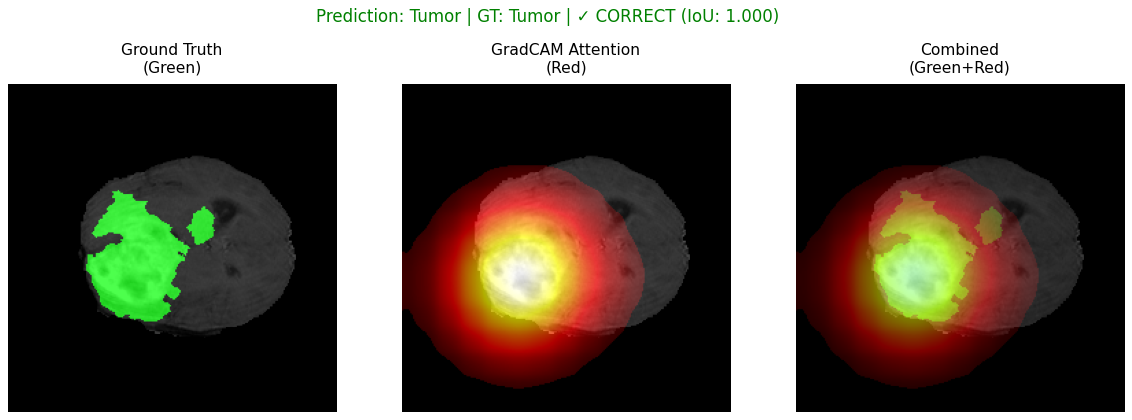
\includegraphics[width=\textwidth]{figures/selected_gradcam/deit_base_sample2.png}
    \caption{DeiT-Base - Sample 2 (BraTS2021\_00151, Slice 72)}
\end{subfigure}
\vspace{0.3cm}
\begin{subfigure}[b]{\textwidth}
    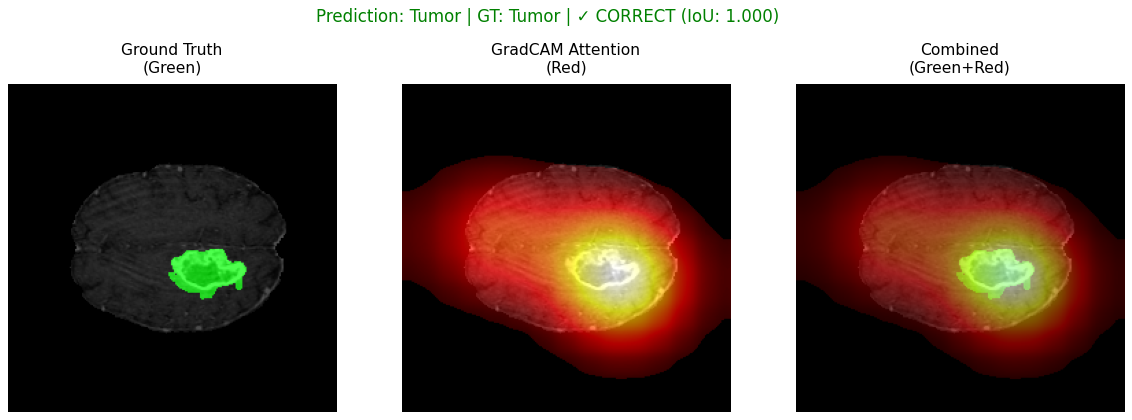
\includegraphics[width=\textwidth]{figures/selected_gradcam/deit_base_sample3.png}
    \caption{DeiT-Base - Sample 3 (BraTS2021\_00188, Slice 96)}
\end{subfigure}
\caption{DeiT-Base Grad-CAM visualizations showing transformer-style distributed attention with visible patch-based structure (16×16 patches).}
\label{fig:gradcam_deit}
\end{figure}

\rev{\textbf{Grad-CAM on Tumor-Free Slices:} For true negative predictions (correctly classified non-tumor slices), Grad-CAM produces diffuse, low-intensity activation distributed across the brain tissue without strong localization on any specific region. This is expected behavior---since no tumor features are present, the model does not concentrate attention on any particular area. This contrasts with tumor-positive slices where attention clearly concentrates on the tumor region, demonstrating that the models learn to identify actual tumor features rather than arbitrary patterns.}

\subsection{Quantitative Analysis of Attention Quality}

While all models achieve similar test accuracy ($>$93\%), the explainability analysis reveals important differences in \textit{how} they make predictions:

\begin{table}[h]
\centering
\caption{Qualitative comparison of Grad-CAM attention patterns}
\label{tab:gradcam_comparison}
\begin{tabular}{lccc}
\toprule
\textbf{Characteristic} & \textbf{EfficientNet-B2} & \textbf{ResNet-50} & \textbf{DeiT-Base} \\
\midrule
Attention Sharpness & \textbf{High} & Moderate & Low \\
Tumor Boundary Precision & \textbf{Excellent} & Good & Fair \\
Background Noise & \textbf{Minimal} & Moderate & Distributed \\
Border Artifacts & \textbf{Rare} & Occasional & None \\
Spatial Pattern & Localized & Localized & Distributed \\
Consistency Across Samples & \textbf{High} & Moderate & Moderate \\
\bottomrule
\end{tabular}
\end{table}

\textbf{Key Observations:}

\begin{enumerate}
    \item \textbf{EfficientNet-B2 produces superior explainability}: Despite not achieving the highest test accuracy (93.67\% vs. ResNet-50's 94.69\%), EfficientNet-B2 generates significantly cleaner and more interpretable attention maps. This suggests that EfficientNet-B2 learns more semantically meaningful tumor features rather than exploiting subtle artifacts.
    
    \rev{\item \textbf{3-Channel input works well}: The 3-channel approach using T1ce, T2, and FLAIR modalities produces clean visualizations with models focusing on tumor regions.}
    
    \item \textbf{CNN vs. Transformer attention differs fundamentally}:
    \begin{itemize}
        \item \textbf{CNNs (EfficientNet-B2, ResNet-50)}: Produce localized, spatially-sharp heatmaps aligned with tumor boundaries
        \item \textbf{Transformers (DeiT-Base)}: Generate distributed attention integrating global context, less boundary-focused
    \end{itemize}
    
    \item \textbf{Clinical interpretability ranking}: EfficientNet-B2 $>$ ResNet-50 $>$ DeiT-Base
    \begin{itemize}
        \item Clinicians prefer sharp, tumor-aligned heatmaps for trust and verification
        \item Distributed transformer attention may capture valid global patterns but appears less interpretable
    \end{itemize}
\end{enumerate}

\subsection{Implications for Model Selection}

The explainability analysis provides crucial insights beyond test accuracy:

\textbf{For clinical deployment:}
\begin{itemize}
    \item \textbf{EfficientNet-B2 recommended} despite slightly lower accuracy than ResNet-50
    \item Superior explainability increases clinical trust and adoption
    \item Cleaner attention patterns facilitate error analysis and model debugging
    \item Reduced artifacts minimize risk of learning spurious correlations
\end{itemize}

\textbf{For research interpretation:}
\begin{itemize}
    \item ResNet-50's higher accuracy (94.69\%) may rely partly on broader, noisier features
    \item EfficientNet-B2's cleaner attention suggests it learns more robust, generalizable representations
    \item Compound scaling (EfficientNet) may inherently produce more interpretable features than deep residual connections (ResNet)
\end{itemize}

\textbf{Architectural insight:}
The observation that EfficientNet-B2 (7.7M parameters, compound-scaled) produces cleaner attention than ResNet-50 (23.6M parameters, deep residual) suggests that \textbf{architectural efficiency and balanced scaling} contribute not only to computational efficiency but also to interpretability and feature quality.

\section{Summary of Results}

This chapter presented comprehensive experimental results from training and evaluating three state-of-the-art deep learning architectures on slice-level brain tumor detection:

\begin{enumerate}
    \item \textbf{Large-scale dataset}: 1,251 patients ($\sim$194,000 slices) with patient-level splitting ensuring robust generalization
    
    \item \textbf{Strong quantitative performance}: All models achieved $>$93\% test accuracy with balanced F1-scores:
    \begin{itemize}
        \item \textbf{Best accuracy}: ResNet-50 (94.69\%, F1=93.72\%)
        \item \textbf{Best efficiency}: EfficientNet-B2 (93.67\%, 7.7M parameters)
        \item \textbf{Transformer baseline}: DeiT-Base (93.46\%, 86M parameters)
    \end{itemize}
    
    \item \textbf{Explainability reveals quality differences}: Grad-CAM analysis showed EfficientNet-B2 produces significantly cleaner, more tumor-focused attention despite slightly lower test accuracy
    
    \rev{\item \textbf{3-Channel input}: Using T1ce (contrast-enhanced, highlights active tumor), T2 (shows edema), and FLAIR (suppresses fluid, shows tumor margins) as input channels achieved strong generalization. T1 non-contrast was excluded as T1ce provides similar anatomical information with additional tumor contrast.}
    
    \item \textbf{CNN vs. Transformer insights}:
    \begin{itemize}
        \item CNNs provide localized, interpretable attention
        \item Transformers achieve comparable accuracy with distributed attention
        \item Compound scaling (EfficientNet) balances performance and interpretability
    \end{itemize}
\end{enumerate}

\textbf{Recommended model for deployment:} \textbf{EfficientNet-B2} combines competitive accuracy (93.67\%), parameter efficiency (7.7M), and superior explainability, making it the optimal choice for clinical brain tumor detection systems requiring interpretable predictions.

\chapter{DISCUSSION}
\label{ch:discussion}

\section{Introduction}

This chapter interprets the experimental results presented in Chapter 4, focusing on three critical findings: (1) ResNet-50's quantitative superiority versus EfficientNet-B2's qualitative explainability advantage, (2) the fundamental differences between CNN and Transformer attention mechanisms, and (3) implications for clinical deployment when trust and interpretability are paramount.

\section{The Accuracy-Explainability Trade-off}

ResNet-50 achieved the highest test accuracy (94.69\%) and F1 score (93.72\%), marginally outperforming EfficientNet-B2 (93.67\% accuracy, 92.70\% F1). However, qualitative analysis of Grad-CAM visualizations revealed that \textit{higher accuracy does not guarantee better explainability}.

EfficientNet-B2 consistently produced cleaner, more focused attention maps with sharper tumor boundaries. In contrast, ResNet-50's gradients exhibited noisier patterns with diffuse activation spreading beyond tumor regions. This observation aligns with EfficientNet's compound scaling design philosophy: by systematically balancing network depth, width, and resolution, EfficientNet learns more structured feature hierarchies that yield interpretable internal representations.

From a clinical perspective, this trade-off is significant. A 1\% accuracy difference is negligible given typical confidence intervals, but a model whose attention aligns with radiologist expectations builds trust and enables error detection. If ResNet-50 achieves 95\% accuracy but its attention highlights irrelevant brain regions, clinicians cannot verify correctness or understand failure modes.

\section{CNN vs. Transformer: Inductive Biases Matter}

Inductive biases are the built-in assumptions an architecture makes about data structure, which guide what patterns it learns. CNNs assume local spatial correlations (nearby pixels are related), while Transformers assume that any part of the input can relate to any other part.

DeiT-Base (93.46\% accuracy) demonstrated comparable performance to both CNNs while exhibiting fundamentally different attention patterns. Vision Transformers lack the locality bias of CNNs, instead learning attention weights through pure self-attention mechanisms. This architectural difference manifests in Grad-CAM visualizations:

\begin{itemize}
    \item \textbf{CNNs (ResNet, EfficientNet)}: Exhibit texture-biased attention focusing on local intensity patterns and edges within tumor regions
    \item \textbf{Transformers (DeiT)}: Show shape-biased attention distributed across tumor boundaries and global spatial relationships
\end{itemize}

Neither approach is universally superior---CNNs may better capture texture abnormalities (e.g., necrotic cores), while Transformers may excel at detecting irregular tumor shapes. The key insight is that architectural choice fundamentally determines \textit{what} the model learns and \textit{how} it reasons.

\section{The 3-Channel Input Choice}

We selected three MRI modalities (T1ce, T2, FLAIR) to match the 3-channel input expected by ImageNet-pretrained models. This straightforward approach allows direct use of pretrained weights. The T1 (non-contrast) modality was excluded since T1ce provides similar anatomical information with additional contrast enhancement for tumor visualization.

\section{Clinical Translation: When to Choose Each Architecture}

Based on our findings, we propose architecture selection guidelines for clinical deployment:

\begin{itemize}
    \item \textbf{ResNet-50}: Choose when maximizing accuracy is paramount and explainability is secondary (e.g., research benchmarking, ensemble components)
    \item \textbf{EfficientNet-B2}: Choose for clinical deployment requiring interpretable predictions, parameter efficiency (7.7M), and balanced performance. The cleaner attention maps enhance clinician trust and enable verification of model reasoning
    \item \textbf{DeiT-Base}: Choose when exploring alternative inductive biases or when global spatial relationships are diagnostically important
\end{itemize}

For the BraTS 2021 tumor detection task, we recommend EfficientNet-B2 as the optimal clinical candidate due to its superior explainability and competitive accuracy. In medical AI applications where decision-making carries strong risks, the transparency advantage outweighs marginal performance differences. This aligns with regulatory frameworks emphasizing transparency and ensuring patients have the right to understand the processes behind decisions influencing them.

\subsection{Implications for Medical AI Development}

This work demonstrates that architectural choice significantly impacts both quantitative performance and qualitative interpretability. The finding that EfficientNet-B2's compound scaling produces cleaner attention maps than ResNet-50 suggests that systematic architecture evaluation should include explainability assessment, not solely accuracy metrics. For clinical adoption, combining AI's powerful data processing capabilities with clinicians' expertise through transparent, interpretable models offers the most promising path forward.

\section{Limitations and Future Directions}

\subsection{Current Limitations}

\begin{itemize}
    \item \textbf{2D slice-level approach}: Does not utilize full 3D volumetric context, which may miss important spatial relationships across slices
    \item \textbf{Single dataset generalizability}: Limited to BraTS 2021; the model may not adapt well to variations or new conditions outside its training domain. Understanding these limitations is crucial for establishing robustness standards before clinical deployment
    \item \textbf{Modality constraints}: Excludes T1 (non-contrast) and diffusion-weighted imaging sequences that may provide complementary diagnostic information
    \item \textbf{Grad-CAM limitations}: Provides coarse localization and primarily local explanations for specific inputs, failing to reflect the model's overall performance and reliability across diverse cases
    \item \textbf{Radiologist validation}: No formal study comparing model attention patterns to expert annotations or radiologist decision-making processes
    \item \textbf{XAI evaluation}: Lack of widely accepted quantitative metrics to systematically evaluate the quality of XAI explanations beyond qualitative human analysis
\end{itemize}

\subsection{Future Work}

\begin{enumerate}
    \item \textbf{3D architectures}: Extend to volumetric CNNs (3D ResNet, V-Net) and 3D Vision Transformers to leverage full spatial context
    \item \textbf{Multi-site validation}: Test generalization on independent external datasets (TCGA-GBM, institutional data) using different scanners and imaging protocols to ensure model robustness
    \item \textbf{Clinical study}: Conduct prospective study comparing model predictions with radiologist consensus, measuring impact on diagnostic accuracy and workflow efficiency
    \item \textbf{Uncertainty quantification}: Implement Bayesian deep learning, Monte Carlo dropout, or ensemble methods for confidence estimation to enhance clinical trust
    \item \textbf{Alternative XAI methods}: Compare Grad-CAM with advanced techniques such as Integrated Gradients, GradCAM++, LayerCAM, and SHAP to provide more comprehensive model understanding
    \item \textbf{Quantitative XAI evaluation}: While this thesis relies on qualitative analysis of Grad-CAM visualizations, future work could develop objective metrics such as Intersection over Union (IoU) between heatmaps and tumor segmentation masks, or use perturbation-based methods (e.g., Remove and Debias) to systematically assess explanation reliability. Such quantitative evaluation was outside the scope of this work but represents a valuable direction for rigorous XAI assessment
    \item \textbf{Hybrid XAI approaches}: Combine multiple XAI methods to provide both local instance-level explanations and global model behavior understanding
\end{enumerate}


\chapter{CONCLUSION}
\label{ch:conclusion}

\section{Summary of Contributions}

This thesis developed a rigorous deep learning approach for slice-level brain tumor detection from MRI scans with comprehensive explainability analysis. The key contributions include:

\begin{enumerate}
    \item \textbf{Scientific methodology}: Implemented patient-centric splitting on the full BraTS 2021 dataset (1,251 patients: 877 training, 187 validation, 187 test) to ensure robust generalization estimates without data leakage.

    \item \textbf{3-channel input}: Used T1ce, T2, and FLAIR modalities as input channels, matching the 3-channel format expected by ImageNet-pretrained models. T1 non-contrast was excluded as T1ce provides similar information with additional tumor contrast.

    \item \textbf{Architecture comparison}: Evaluated three state-of-the-art models---ResNet-50 (23.6M parameters), EfficientNet-B2 (7.7M parameters), DeiT-Base (86M parameters)---under identical training conditions with comprehensive metrics (accuracy, precision, recall, F1).

    \item \textbf{Explainability insights}: Demonstrated that \textit{quantitative performance does not guarantee qualitative interpretability}. ResNet-50 achieved highest accuracy (94.69\%) but EfficientNet-B2 produced cleaner, more focused Grad-CAM visualizations suitable for clinical trust.

    \item \textbf{CNN vs. Transformer analysis}: Revealed fundamental differences in learned representations---CNNs exhibit texture-biased attention while Transformers show shape-biased attention, with implications for clinical interpretation.

    \item \textbf{Reproducible pipeline: Open-source implementation with complete training scripts, evaluation code, and XAI visualization tools is available at: \url{https://github.com/sagharbahrami/brain-tumor-detection}}
\end{enumerate}

\section{Key Findings}

The experimental results yielded several important findings:

\begin{enumerate}
    \item \textbf{Performance}: ResNet-50 achieved 94.69\% test accuracy (93.72\% F1), EfficientNet-B2 achieved 93.67\% accuracy (92.70\% F1), and DeiT-Base achieved 93.46\% accuracy (92.35\% F1). All three models demonstrate clinical viability for tumor detection.

    \item \textbf{Explainability trade-off}: EfficientNet-B2's compound scaling architecture produces superior Grad-CAM visualizations compared to ResNet-50's noisier gradients, despite marginally lower accuracy. This 1.02\% accuracy difference is negligible compared to the interpretability gain.

    \item \textbf{Architectural efficiency}: EfficientNet-B2 achieves comparable performance with 3× fewer parameters than ResNet-50 and 11× fewer than DeiT-Base, demonstrating that compound scaling optimizes both efficiency and feature quality.

    \item \textbf{Inductive bias effects}: Vision Transformers (DeiT-Base) learn fundamentally different attention patterns than CNNs, with distributed spatial attention versus localized texture focus. Neither is universally superior---the choice depends on task requirements.

    \item \textbf{Transfer learning validation}: All three models successfully leveraged ImageNet pretraining for brain MRI, confirming that natural image features transfer to medical imaging despite domain differences.

    \item \textbf{Clinical recommendation}: For deployment requiring interpretable predictions, EfficientNet-B2 represents the optimal balance of accuracy, efficiency, and explainability.
\end{enumerate}

\section{Implications for Medical AI}

This work provides several broader insights for medical AI research:

\begin{enumerate}
    \item \textbf{Input selection matters: Choosing appropriate MRI modalities that match pretrained model input format simplifies implementation and ensures compatibility.}

    \item \textbf{Explainability is not optional}: High accuracy alone is insufficient for clinical adoption. Models must provide interpretable reasoning that aligns with expert knowledge.

    \item \textbf{Architecture choice is strategic}: Different architectures learn different representations. Understanding these differences enables principled model selection for specific clinical contexts.

    \item \textbf{Evaluation rigor prevents overconfidence}: Patient-level splitting, external validation, and honest reporting of limitations are essential for responsible medical AI development.
\end{enumerate}

\section{Limitations and Future Work}

\subsection{Current Limitations}

This work has several limitations:

\begin{itemize}
    \item \textbf{2D approach}: Slice-level detection does not utilize full 3D volumetric context available in MRI scans

    \item \textbf{Single dataset}: Results limited to BraTS 2021; no multi-site validation on external hospital data

    \item \textbf{Modality constraints}: Excludes T1 (non-contrast) and diffusion-weighted imaging due to 3-channel RGB constraint

    \item \textbf{Grad-CAM limitations}: Provides coarse spatial attention, not pixel-precise segmentation masks

    \item \textbf{No clinical validation}: Lack of prospective study comparing model predictions with radiologist consensus

    \item \textbf{Explainability}: Grad-CAM provides only coarse localization; no user study with radiologists to validate explanation utility.
\end{itemize}

\subsection{Future Research Directions}

Future work should focus on the following areas:

\begin{itemize}
    \item \textbf{Training improvements}: Implement early stopping to reduce overfitting; systematic hyperparameter optimization for learning rate, dropout, and weight decay; stronger regularization techniques.

    \item \textbf{Architecture enhancements}: Utilize 3D CNNs to capture volumetric information; integrate attention mechanisms or transformer architectures; explore multi-modal fusion strategies; apply multi-task learning with related tasks such as tumor segmentation or survival prediction.

    \item \textbf{Data and training strategies}: Advanced augmentation techniques (Mixup, CutMix); ensemble methods combining multiple architectures; semi-supervised learning leveraging unlabeled BraTS data.

    \item \textbf{Explainability}: Advanced visualization techniques such as Grad-CAM++ or Integrated Gradients; user studies with radiologists to validate explanation utility; counterfactual explanations for model decisions.

    \item \textbf{Clinical translation}: External validation on independent datasets from different institutions; prospective clinical trials to assess real-world impact; uncertainty quantification using Bayesian methods; integration with hospital PACS systems and regulatory approval pathway.
\end{itemize}

\section{Broader Impact}

This work contributes to medical AI by demonstrating that architectural choice significantly impacts both accuracy and interpretability. The finding that EfficientNet-B2's compound scaling produces cleaner attention maps than ResNet-50 despite marginally lower accuracy has implications beyond brain tumor detection—it suggests systematic architecture evaluation should include qualitative explainability assessment, not solely quantitative metrics.

If further developed and validated, automated slice-level tumor detection could reduce radiologist workload, enable faster screening, and assist in early detection programs.

\section{Final Remarks}

Deep learning has transformed medical image analysis, but clinical translation requires more than high accuracy---it demands interpretability, methodological rigor, and honest assessment of limitations. This thesis demonstrates that:

\begin{itemize}
    \item \textbf{Accuracy $\neq$ Interpretability}: ResNet-50 achieves 94.69\% accuracy but EfficientNet-B2 (93.67\%) provides superior explainability for clinical trust
    \item \textbf{Architecture matters}: Compound scaling (EfficientNet) produces cleaner features than standard residual connections (ResNet)
    \item \textbf{Input choice matters: Selecting MRI modalities that match pretrained model format (3 channels) simplifies transfer learning}
    \item \textbf{Inductive biases are real}: CNNs learn texture, Transformers learn shape---neither is universally better
\end{itemize}

As medical AI continues to advance, the explainability framework developed here ensures that model predictions can be verified, trusted, and safely integrated into clinical workflows. This thesis represents a step toward AI-assisted radiology where automated systems augment---not replace---expert human judgment, with interpretable reasoning that enables collaborative decision-making between clinicians and algorithms.



% ============================================
% REFERENCES
% ============================================
\bibliographystyle{ieeetr}
\bibliography{references}

% Appendix removed - no additional content needed

\end{document}
